\documentclass[oneside,a4paper,12pt]{book}

\usepackage[spanish]{babel}
\usepackage[utf8]{inputenc}
\usepackage{geometry}
\usepackage{makeidx}
\usepackage{url}
\usepackage{graphicx}
\usepackage{color}
\usepackage{caption}
\usepackage{acronym}
\usepackage{hyphenat}
\usepackage{a4wide}
\usepackage[normalsize]{subfigure}
\usepackage{float}
\usepackage{titlesec}
\usepackage[Lenny]{fncychap}
\usepackage{listings} % para poder hacer uso de "listings" propios (p.ej. códigos)
\usepackage{eurosym} % para poder usar el símbolo del euro con \euro {xx}
\usepackage{hyperref} % TODO: añade la opción hidelinks para imprimirlo (los enlaces no aparecerán resaltados)

% Para que no parta las palabras
\pretolerance=10000

\newcommand{\bigrule}{\titlerule[0.5mm]} \titleformat{\chapter}[display] % cambiamos el formato de los capítulos
{\bfseries\Huge} % por defecto se usaron caracteres de tamaño huge en negrita
{% contenido de la etiqueta 
\titlerule % línea horizontal 
\filright % texto alineado a la derecha 
\Large\chaptertitlename\ % capítulo e índice en tamaño large
\Large % en lugar de 
\Huge \Large\thechapter} 
{0mm} % espacio mínimo entre etiqueta y cuerpo
{\filright} % texto del cuerpo alineado a la derecha
[\vspace{0.5mm} \bigrule] % después del cuerpo, dejar espacio vertical y trazar línea horizontal gruesa
\geometry{a4paper, left=3.5cm, right=2cm, top=3cm, bottom=2cm, headsep=1.5cm}

% Estilos para ilustrar códigos:
\definecolor{code_green}{rgb}{0,0.6,0}
\definecolor{code_gray}{rgb}{0.5,0.5,0.5}
\definecolor{code_mauve}{rgb}{0.58,0,0.82}

\lstset{frame=tb,
  language=C++,
  aboveskip=3mm,
  belowskip=3mm,
  showstringspaces=false,
  columns=flexible,
  basicstyle={\small\ttfamily},
  numbers=none,
  numberstyle=\tiny\color{code_gray},
  keywordstyle=\color{blue},
  commentstyle=\color{code_green},
  stringstyle=\color{code_mauve},
  breaklines=true,
  breakatwhitespace=true,
  tabsize=3
}

\lstset{frame=tb,
  language=Python,
  aboveskip=3mm,
  belowskip=3mm,
  showstringspaces=false,
  columns=flexible,
  basicstyle={\small\ttfamily},
  numbers=none,
  numberstyle=\tiny\color{code_gray},
  keywordstyle=\color{blue},
  commentstyle=\color{code_green},
  stringstyle=\color{code_mauve},
  breaklines=true,
  breakatwhitespace=true,
  tabsize=3
}


\definecolor{maroon}{rgb}{0.5,0,0}
\definecolor{darkgreen}{rgb}{0,0.5,0}
\definecolor{gray}{rgb}{0.4,0.4,0.4}

\lstdefinelanguage{XML}
{
  numbers=none,
  numberstyle=\tiny\color{code_gray},
  stepnumber=1,
  basicstyle=\ttfamily,
  morestring=[s]{"}{"},
  morecomment=[s]{?}{?},
  morecomment=[s]{!--}{--},
  commentstyle=\color{darkgreen},
  moredelim=[s][\color{black}]{>}{<},
  moredelim=[s][\color{red}]{\ }{=},
  stringstyle=\color{blue},
  identifierstyle=\color{maroon}
}

\DeclareCaptionType{code}[Código][Listado de códigos]




% Bibliografa
\usepackage[spanish]{babel}
\usepackage[utf8]{inputenc}
\usepackage[backend=biber]{biblatex}
\bibliography{bibliografia}


\makeindex

\begin{document}


\thispagestyle{empty}

\begin{titlepage}
	\begin{center}
		\vspace*{3mm}
		\begin{center}
			
\includegraphics[width=0.4\linewidth]{imagenes/logo.jpg}
		\end{center}
		\vspace{6.0mm}
		
		\fontsize{15.5}{14}\selectfont ESCUELA TÉCNICA SUPERIOR DE INGENIERÍA DE TELECOMUNICACIÓN
		\vspace{13mm}
		
		\fontsize{14}{14}\selectfont GRADO EN INGENIERÍA DE ROBÓTICA SOFTWARE
		
		\vspace{70pt}
		
		\fontfamily{lmss}\fontsize{15.7}{14}\selectfont \textbf{TRABAJO FIN DE GRADO} 
		
		\vspace{20mm}
		\begin{LARGE}
			Ejercicios Sigue-Persona para la plataforma académica Robotics Academy, usando un robot real y simulado en ROS2
		\end{LARGE}
		
		\vspace{20mm}
		
		\begin{large}
			Autor: Carlos Caminero Abad
			
			Tutor: Dr. Jose María Cañas Plaza
			
			\vspace{10mm}
		\end{large}
		\begin{normalsize}
			Curso académico 2021/2022		
		\end{normalsize}
		\vspace{10mm}
		
	\end{center}
	
\end{titlepage}

\thispagestyle{empty}

\pagenumbering{roman}
\chapter*{Agradecimientos}

El final ha llegado. Escribiendo estas palabras, me acuerdo de todas aquellas personas que han estado presentes a lo largo de mi vida y de este viaje, y que gracias a ellos estoy aquí, a unos días de presentar un proyecto que marcará el final de una de las etapas de mi vida y el principio de otra.\\

Quisiera dar las gracias a mis padres y a mi hermano. Siempre han estado conmigo, apoyándome y ayudándome cuando lo he necesitado. Gracias a mis padres, conocí este grado universitario, y haberlo elegido ha sido una de las mejores decisiones que he tomado en mi vida. Siempre les estaré agradecido.\\

Quisiera agradecer a mis amigos de Yepes por todos los buenos momentos compartidos. Por todas aquellas cenas, en las que nos desahogábamos de nuestros problemas y por todo el apoyo y ánimo que me han transmitido. Es un placer compartir esta vida con gente tan excelente como ellos.\\

Por otra parte, agradezco a mis compañeros de clase por estos cuatro años que, a pesar de compartir duras y difíciles experiencias como la pandemia, también he podido compartir buenos momentos de satisfacción y alegría con ellos.\\ 

Por último, quería agradecer a todos mis profesores por su dedicación e interés por la enseñanza que me han transmitido y en especial, a mi tutor Jose María, por haber estado orientándome a lo largo de todos estos meses dedicados al proyecto. Gracias por toda tu dedicación y animos, y por tu ayuda cuando me encontraba bloqueado por el camino. Ha sido todo un honor haberte tenido como profesor y como tutor.\\

\begin{center}
	¡Muchas gracias a todos!
\end{center}

\chapter*{Resumen}

La Robótica es un sector en constante crecimiento. Cada vez es más importante el perfil del Ingeniero en Robótica Software para la programación de Robots y Automatismos en esta nueva era digital. Por ello, es necesario la correcta formación del Ingeniero a través de la accesibilidad y disponibilidad de los recursos educativos que fomentarán su aprendizaje autodidacta.\\

El objetivo del siguiente Trabajo Fin de Grado (TFG) es desarrollar dos nuevos ejercicios educativos para la plataforma de enseñanza universitaria Robotics Academy consistentes en programar un robot modelo TurtleBot2 de Yujin para que sea capaz de seguir a una persona tanto en un entorno real como en un entorno simulado (un hospital). Con ello, los alumnos y otros usuarios adquirirán las destrezas necesarias para la programación de una tarea muy solicitada en la Robótica de Servicio. Aprenderán a seguir a una persona usando Redes Neuronales que ayudarán a la detección visual de personas en imágenes\\

La incorporación de estos dos nuevos ejercicios se aplica a una nueva rama de desarrollo para la plataforma Robotics Academy que usa la distribución ROS2 Foxy. Además, se ha logrado la migración y adaptación del modelo simulado del Turtlebot2 de ROS Noetic a ROS2 Foxy para futuros usos. Se ha preparado la página web operativa correspondiente a cada ejercicio y se han desarrollado las respectivas soluciones de referencia que combinan percepción visual robusta y navegación con el algoritmo VFF.

\cleardoublepage

\chapter*{Acrónimos\markboth{Acrónimos}{Acrónimos}}

\begin{acronym}
	\acro{CNN}{\emph{Convolutional Neural Network}}
	\acro{CPU}{\emph{Central Processing Unit}}
	\acro{CSS}{\emph{Cascading Style Sheets}}
	\acro{DNN}{\emph{Deep Neural Network}}
	\acro{FSM}{\emph{Finite State Machine}}
	\acro{GPU}{\emph{Graphics Processing Unit}}
	\acro{GUI}{\emph{Graphical User Interface}}
	\acro{HAL}{\emph{Hardware Abstraction Layer}}
	\acro{HTML}{\emph{HiperText Markup Language}}
	\acro{HTTP}{\emph{HiperText Transfer Protocol}}
	\acro{IA}{\emph{Inteligencia Artificial}}
	\acro{LIDAR}{\emph{Laser Imaging Detection and Ranging}}
	\acro{ML}{\emph{Machine Learning}}
	\acro{PID}{\emph{Proportional-Integral-Derivative}}
	\acro{RNA}{\emph{Redes Neuronales Artificiales}}
	\acro{R-CNN}{\emph{Region-based Convolutional Neural Network}}
	\acro{ROS}{\emph{Robot Operating System}}
	\acro{UDP}{\emph{User Datagram Protocol}}
	\acro{URDF}{\emph{Unified Robot Description Format}}
	\acro{USB}{\emph{Universal Serial Bus}}
	\acro{XML}{\emph{eXtensible Markup Language}}
\end{acronym}

\cleardoublepage

\tableofcontents

\listoffigures

\listofcodes

\pagestyle{empty}

\cleardoublepage


\mainmatter

\chapter{Introducción}
\label{cap:capitulo1}
\setcounter{page}{1}

La tarea Sigue-Personas es una de las más empleadas y solicitadas en los Robots de Servicio para multitud de sectores que incorporan soluciones robóticas. El siguiente TFG propone desarrollar dos nuevos ejercicios para la plataforma Unibotics con el objetivo de que los usuarios programen un robot Turtlebot2 tanto en simulado como en real para que realice dicha tarea.\\

Este primer capítulo trata de presentar el estado actual de varios campos de la Robótica que están directamente relacionados con este proyecto para poner en contexto al lector y facilitar su lectura.\\

Por un lado presentaremos la Robótica Móvil, un sector de la robótica que está en constante crecimiento y muy presente en la Robótica de Servicio; por otra parte, introduciremos las Redes Neuronales, un avance significativo en IA que ha permitido realizar aplicaciones muy robustas basadas en la percepción y el razonamiento; y por último hablaremos de la Robótica Educativa, e introduciremos varias plataformas como TheConstruct, Robotics Academy, o Unibotics siendo estas dos últimas las que incorporarán el ejercicio educativo Sigue-Persona.



\section{Robótica Móvil}
\label{sec:robotica_movil}

La robótica es la ciencia que engloba varias ramas tecnológicas o disciplinas, con el objetivo de diseñar máquinas (``robots'') que sean capaces de realizar tareas automatizadas o de simular el comportamiento humano o animal, en función de la capacidad de su software. \cite{revistaderobots}. Su término se remonta a la obra de ciencia ficción escrita por Isaac Asimov: Yo, Robot. (1950)\\

Una vez que la robótica emerge a partir de mediados del siglo XX, surgen 2 sectores: la Robótica Industrial y la Robótica de Servicio. Los \textbf{Robots industriales} se encargan de realizar tareas automatizadas y muy repetitivas en entornos industriales, donde el entorno es controlado. Los \textbf{Robots de Servicio} son aquellos que realizan tareas útiles para el ser humano proporcionándole un servicio. Destacan los robots móviles que permiten desplazarse de un sitio a otro, sin embargo el entorno en el que se enfrentan es bastante heterogéneo, por tanto su software tiene que ser muy robusto para adaptarse correctamente a los cambios.\\

Un \textbf{robot móvil} un sistema electromecánico capaz de desplazarse de ma­nera autónoma sin estar sujeto físicamente a un solo punto. Posee sensores que permiten monitorear a cada momento su posición relativa a su punto de origen (odometría) y a su punto de destino. Normalmente su control es en lazo cerrado. Se clasifican en robots móviles de \textbf{locomoción con ruedas}, \textbf{locomoción con patas} y \textbf{locomoción con orugas}.  Los primeros son más fáciles de controlar pero no se adaptan bien a muchas superficies, sin embargo los robots con patas (cuadrúpedos o bípedos) se adaptan muy bien a distintas superficies pero requieren varios controladores para mantener su equilibrio tanto estático como dinámico.




\subsection{Evolución Histórica}
\label{subsec:evolucion_historica}

Podemos destacar varios hechos importantes a lo largo del siglo XX y principios del XXI que 
marcaron grandes avances en la robótica:

\begin {itemize}
	\item En 1952 aparece la primera máquina de control numérico del MIT que era capaz de automatizar algunas tareas industriales.
	\item En 1961, la compañía Unimates introdujo el primer robot industral en la General Motors.
	\item En 1966, comenzó el desarrollo del primer robot móvil llamado Shakey [Nilsson, 1984]. \ref{fig:shakey}
	\item En los años 70, NASA desarrolló MARS-ROVER, una plataforma móvil que integraba un brazo mecánico, sensores de proximidad, un dispositivo telemétrico láser y cámaras estéreo
	\item En 1997, la NASA envió a Marte un dispositivo móvil llamado Sojourner Rover, para enviar fotografías a la Tierra del planeta rojo. Además, la empresa HONDA sacó el primer humanoide capaz de imitar comportamientos humanos
	\item En 2000, Honda presenta el robot Asimo.
	\item En 2004, Qrio de Sony, un pequeño robot humanoide capaz de correr, bailar, y reconocer caras.
	\item En 2008, SoftBank Robotics presenta el Robot Nao, un robot bípedo dedicado a interactuar con el ser humano y ser muy amigable
	\item En 2013, Boston Dynamics saca a la luz el robot Atlas, un humanoide con actuadores neumáticos. La empresa lo usa para imitar el comportamiento humano llevándolo a otro nivel haciendo acrobacias o incluso parkour.
	\item En 2014, SoftBank Robotics presenta el robot Pepper, robot con forma humana pero se desplaza con ruedas. Se ha usado sobre todo como robot guía, recepcionista y en exhibiciones, sin embargo, fue abandonado en 2021
	\item En 2020, Boston Dynamics saca a la venta el robot cuadrúpedo que imita el comportamiento de un perro llamado Spot, que se usa en algunas fábricas para transportar materiales o realizar tareas de mantenimiento
\end{itemize}

\begin{figure} [h!]
  \begin{center}
    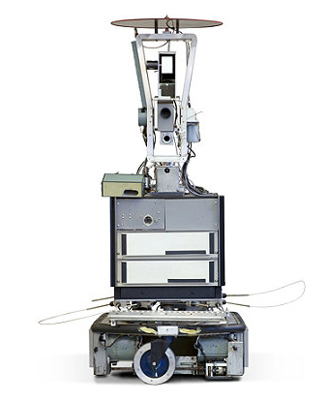
\includegraphics[width=5cm]{imagenes/shakey.jpg}
  \end{center}
  \caption[Shakey (1966-1972)]{Shakey (1966-1972) \cite{shakey-the-robot}.}
  \label{fig:shakey}
\end{figure}\



\subsection{Aplicaciones actuales}
\label{subsec:aplicaciones_actuales}



\section{Redes Neuronales Artificiales (RNA)}
\label{sec:redes_neuronales}

Según \emph{Arthur Samuel}, el Aprendizaje Automático o Machine Learning es el ``campo de estudio que otorga a los ordenadores la capacidad de aprender sin ser programados explícitamente''. Para ello se emplean diversas técnicas dependiendo del objetivo deseado: Regresión Lineal, Regresión Logística, K-NN, K-Means, SVM, Redes Neuronales, Q-Learning, etc.
\\

Cuando incorporamos una RNA, lo que queremos es que nuestro programa o aplicación sepa \textbf{clasificar} unos datos de entrada con su correspondiente salida, habiendo entrenado previamente un modelo computacional inspirado en el cerebro humano. Para ello se le proporciona un set de datos de entrenamiento, donde indicamos, por cada muestra, a qué clase pertenece (Aprendizaje Supervisado). De esta forma, ajustando los valores de unos pesos que se utilizan en el entrenamiento, conseguiremos un nivel de clasificación determinado.\\

Una aplicación de Redes Neuronales es la detección mediante Vision Artificial de objetos. Para ello, se usan modelos de redes de varias capas con un gran número de neuronas (Deep Learning) y de esta forma conseguimos dada una imagen detectar ciertos objetos solicitados como puede ser fruta, coches, utensilios o incluso hasta personas y animales.\\

Típicamente, una Red Neuronal consta de un conjunto de capas formado por varias neuronas que se encuentran interconectadas. Suelen dividirse en 1 capa de entrada, 1 o más capas ocultas y 1 capa de salida. Pero, ¿cómo funciona una neurona?\\

Una neurona, tal y como se muestra en la figura \ref{fig:neurona} está formada pos los siguientes elementos:
\begin{itemize}
	\item \textbf{Valores de Entrada}: Puede ser tanto los valores de las \textbf{características} de cada muestra como la salida de la neurona de una capa anterior.
	\item \textbf{Pesos}: Son unos valores que se optienen al final de la etapa de entrenamiento.
	\item \textbf{Sumatorio}: Esta formado por los productos de los Valores de Entrada por sus correspondientes Pesos
	\item \textbf{Función de Decisión/Activación}: Es una función matemática que se aplica al sumatorio: Lineal, Escalón, Sigmoide, etc
	\item \textbf{Salida}: Es el valor de la función de decisión. Dependiendo de la función de activación usada, la salida será distinta.
\end{itemize}

\begin{figure} [h!]
  \begin{center}
    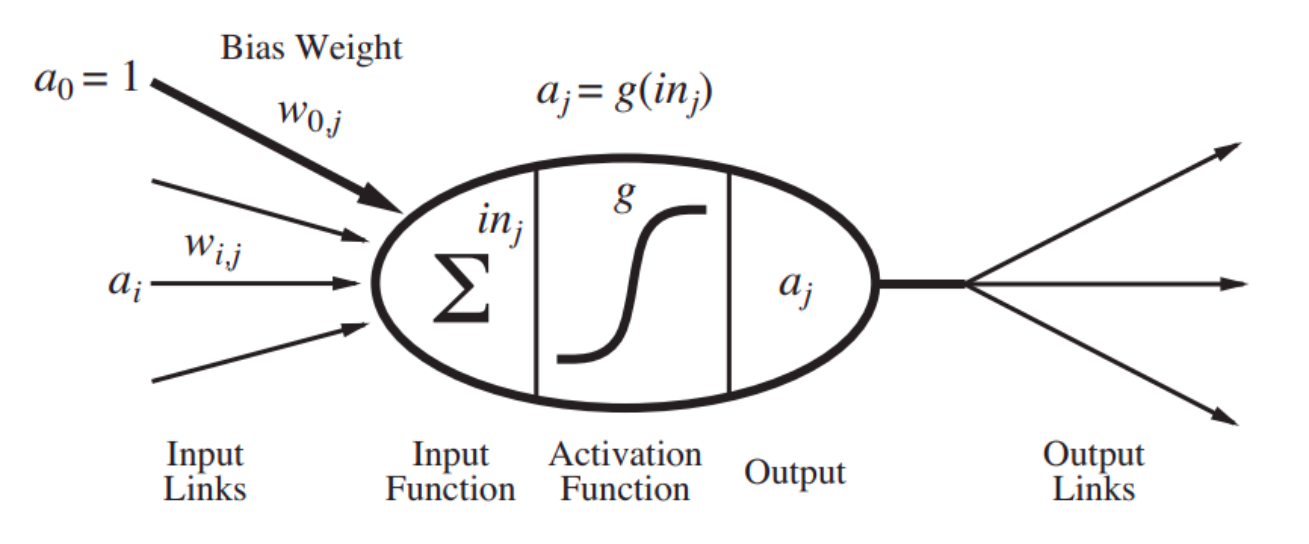
\includegraphics[width=15cm]{imagenes/neurona.png}
  \end{center}
  \caption[Modelo computacional de una neurona]{Modelo computacional de una neurona \cite{AIMA}}
  \label{fig:neurona}
\end{figure}


\subsection{Redes Neuronales Convolucionales (CNN)}
\label{subsec:redes_convolucionales}

\subsection{YOLO}
\label{subsec:yolo}

\subsection{SSD}
\label{subsec:SSD}

\section{Educación en Robótica}
\label{sec:educacion_robotica}

\subsection{Grado en Ingeniería de Robótica Software (URJC, España)}
\label{subsec:grado_robotica_software}
La Universidad Rey Juan Carlos (España) imparte en el campus de Fuenlabrada, el grado en Ingeniería de Robótica Software (primer año: 2018) para enseñar a los futuros ingenieros interesados en este campo a programar la \textbf{inteligencia} de los robots del futuro.\\

Tal y como indica el título del grado, se trata de una carrera universitaria de programación, donde los alumnos abarcarán varios temas como por ejmplo Inteligencia Artificial, visión artificial, programación de lenguajes de alto nivel (C++, Python...), Seguridad, Drones, robots de servicio, robótica industrial, y mucho más. Las clases se imparten tanto en salas de ordenadores con sistemas operativos Linux (distribución Ubuntu) como en el laboratorio de Robótica, donde los alumnos podrán programar directamente robots reales.\\

El robot usado en este Trabajo Fin de Grado es un modelo Turtlebot 2 de Yujin. Consta de una base (kobuki) similar a la de un robot de limpieza con sensores de contaco (bumpers), y un soporte encima que le permite incorporar un RPLIDAR, una cámara, y colocar el portátil del estudiante cuando desarrolla una solución al problema.

\subsection{The Construct}
\label{sec:the_construct}
The Construct es una organización que mantiene una plataforma para aprender robótica con ROS, un framework para programar robots. Imparten varios cursos donde los usuarios acceden a máquinas virtuales con un Linux instalado y todas las dependencias adquiridas. 

\subsection{Robotics Academy}
\label{sec:robotics_academy}
Robotics Academy \cite{robotics-academy} es una colección de ejercicios y desafíos para aprender robótica. Está mantenido por la organización JdeRobot. Sus ejercicios abarcan varios temas: drones, robótica móvil, visión artificial, coches autónomos, robótica industrial, etc. Además es una plataforma Open Source, por lo que cualquier interesado/a puede contribuir desde Github.\\

En sus orígenes, solo se podía ejecutar sobre un sistema operativo Linux, pero desde sus últimas versiones puede ejecutar también sobre Windows y MAC, gracias a la incorporación de plantillas web que se ejecutan en un navegador estableciendo una conexión a través de WebSockets con un contenedor docker que lanza el usuario, permitiendo de esta manera, el despliegue de los ejercicios sobre un sistema operativo virtualizado y con todas sus dependencias ya instaladas.\\

Los usuarios una vez que escogen un ejercicio, lanzan un contenedor docker indicado y automáticamente tienen acceso a una dirección web local donde pueden empezar a programar. La plantilla web incorpora un Editor de Texto y la posibilidad de visualizar un entorno de Gazebo y un terminal mediante una conexión VNC con el contenedor. En la figura \ref{fig:rob-ac-web-template} vemos un ejemplo de plantilla web correspondiente al ejercicio \textit{Follow Person}. La programación se realiza con Python (un lenguaje fácil de entender y aprender, y muy usado en la Robótica).\\

\begin{figure} [h!]
  \begin{center}
    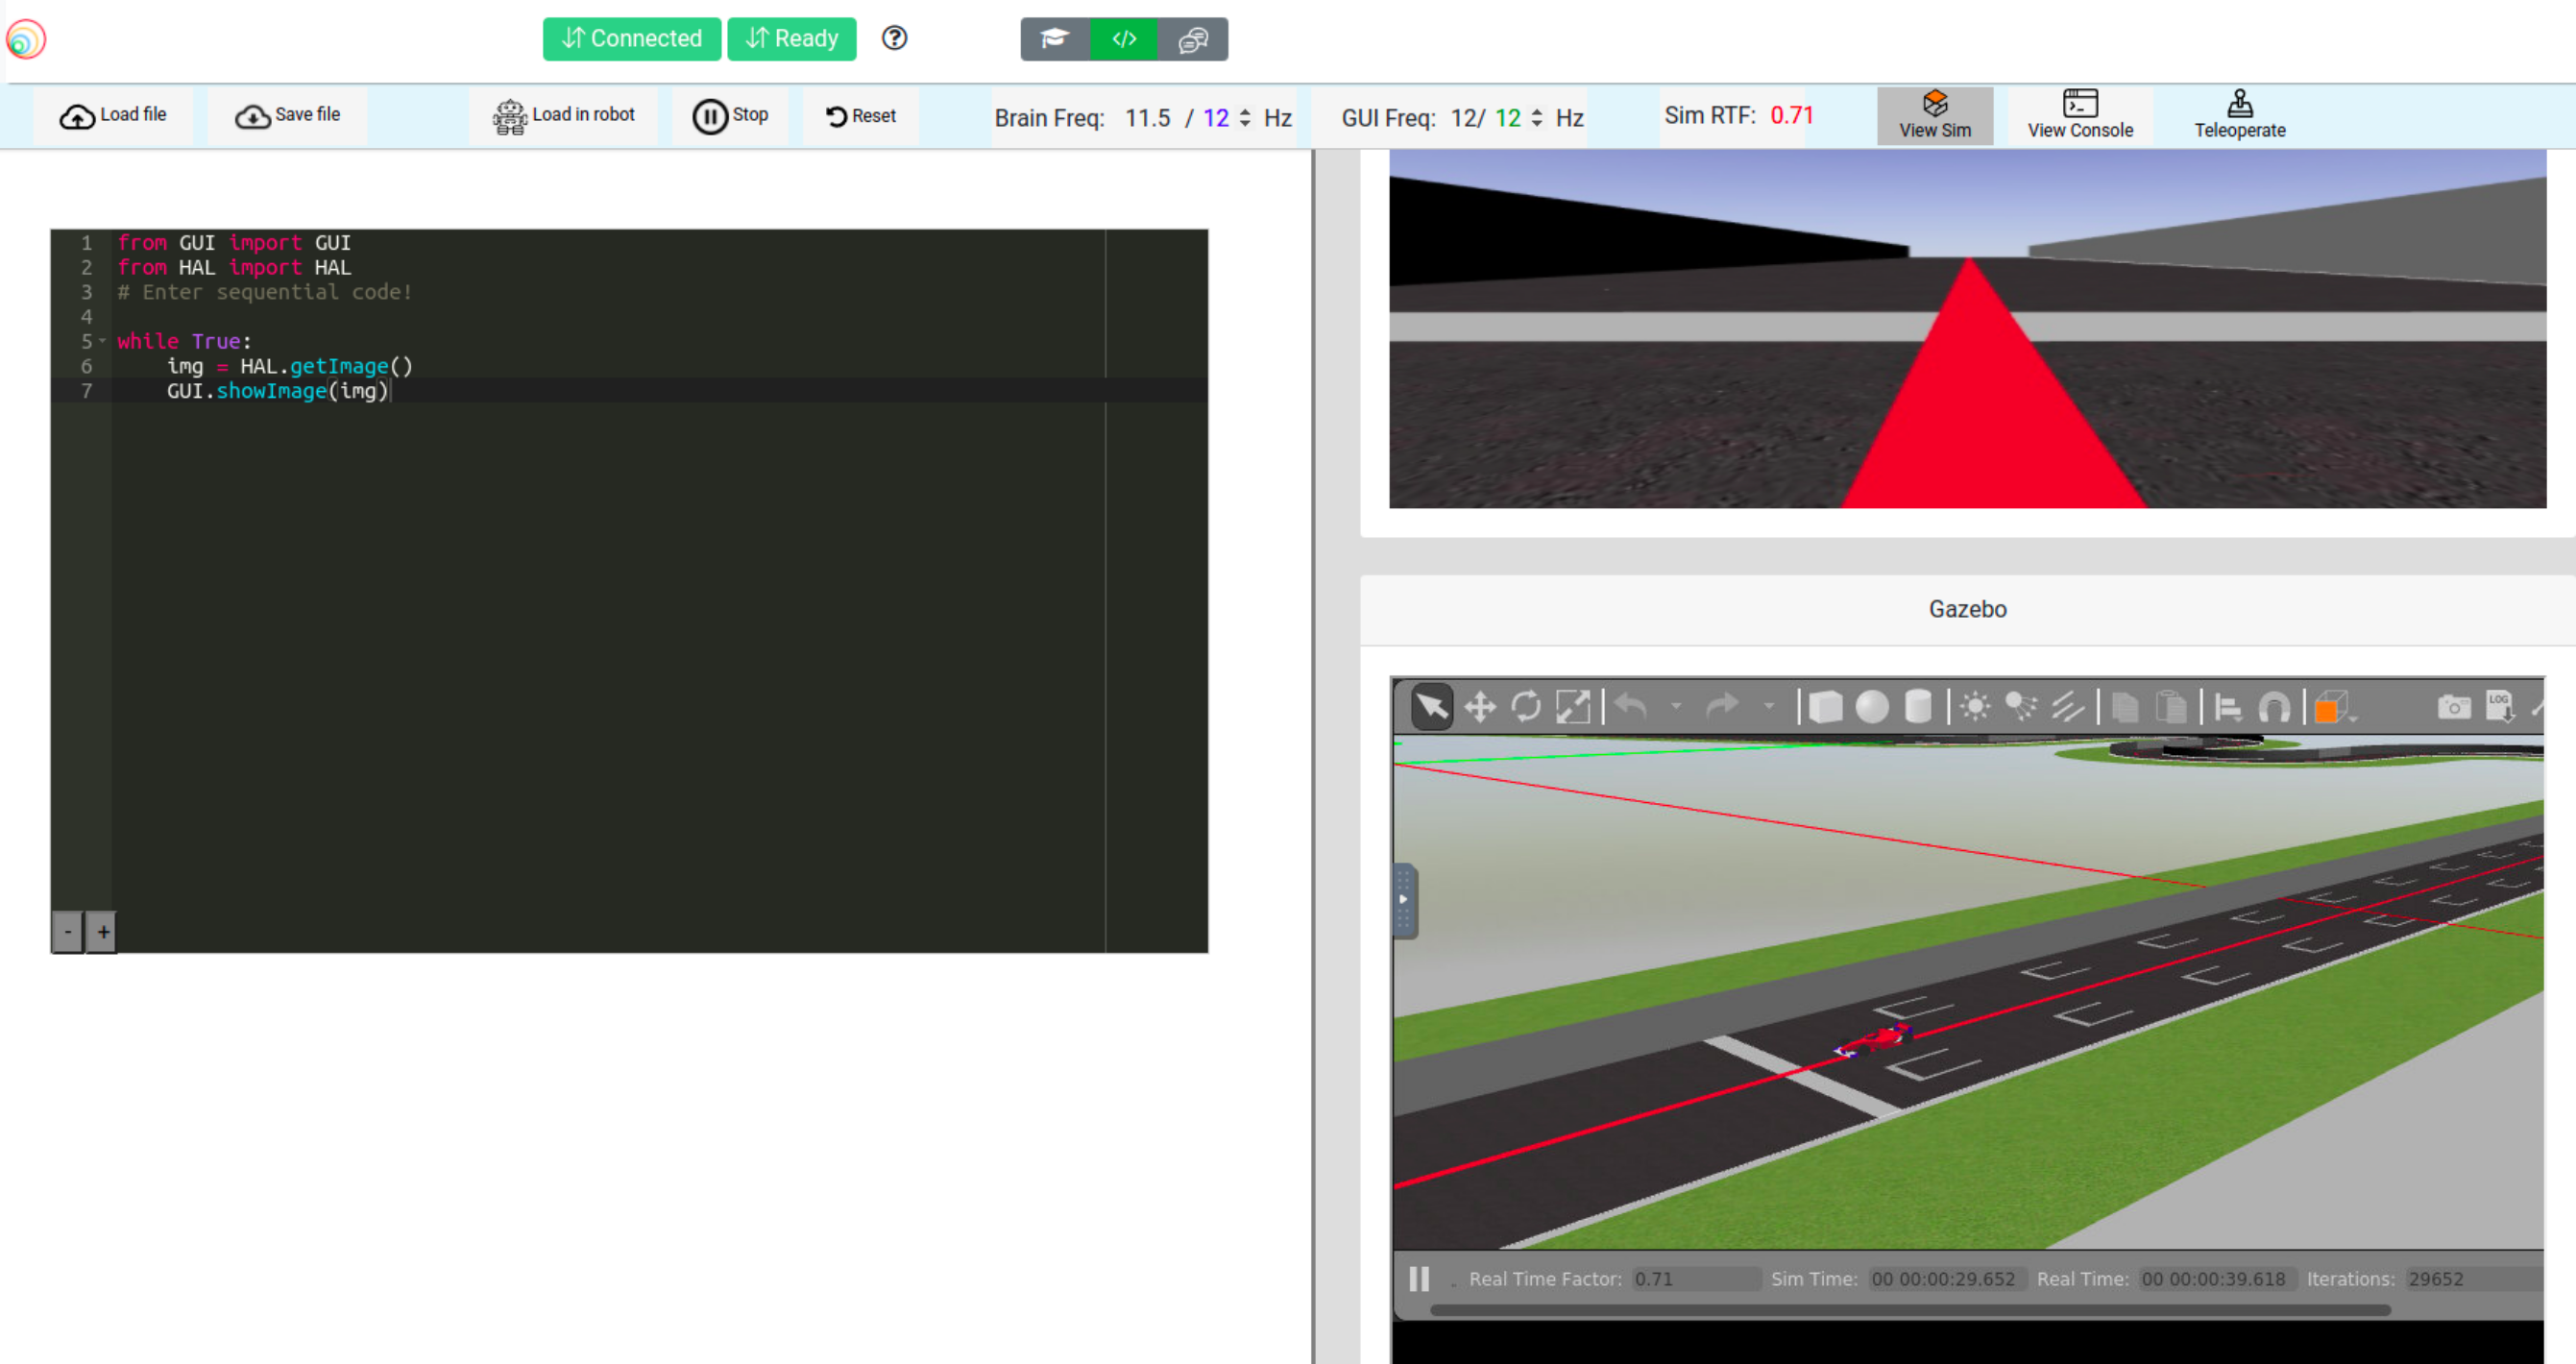
\includegraphics[width=15cm]{imagenes/robotics-academy-web-template.png}
  \end{center}
  \caption[Robotics Academy (Web Template)]{Robotics Academy (Web Template)}
  \label{fig:rob-ac-web-template}
\end{figure}

Una ventaja de usar Robotics Academy, es que permite al usario centrarse única y exclusivamente con el algoritmo que tenga que implementar. Toda la complejidad relacionada con la comunicación con el hardware del robot: motores, laser, cámara, etc. que, por lo general se realiza mediante ROS (un framework para programar Robots) queda encapsulado por 2 módulos: HAL y GUI. De esta manera, el usuario dispone de una API de HAL (Hardware Abstración Layer) para comandar a los actuadores o recibir información de los sensores, y una API de GUI (Graphical User Interface) para visualizar por el navegador información como puede ser una imagen, un mapa o incluso vectores.\\

\subsection{Unibotics}
\label{sec:unibotics}

\textbf{Unibotics} es una plataforma de Robótica que incorpora parte de la coleción de ejercicios de Robotics Academy. Con Unibotics, JdeRobot da un nuevo paso, permitiendo a los usuarios registrarse en un servidor donde pueden guardar sus códigos, acceder cuando deseen, y además, poder contar con la posibilidad de lanzar los ejercicios en un servidor remoto de manera que los usuarios no necesiten instalar docker en sus sistemas operativos.\\

Una vez que el usuario introduce sus credenciales y accede a su sesión, tiene una lista de ejercicios disponibles [Figura \ref{fig:menu-unibotics}], que funcionan de la misma manera que aquellos que proporciona \textit{Robotics Academy}. Actualmente todos los ejercicios disponibles están implementados usando dentro del sistema operativo virtual la distribución ROS Noetic como báse.

Con los 2 nuevos ejercicios Sigue-Personas que explicaremos en este proyecto, pretendemos integrarlos en Unibotics usando ROS Foxy como base. De esta manera, marcaremos un inicio para la migración de varios ejercicios de ROS Noetic a ROS Foxy

\begin{figure} [h!]
  \begin{center}
    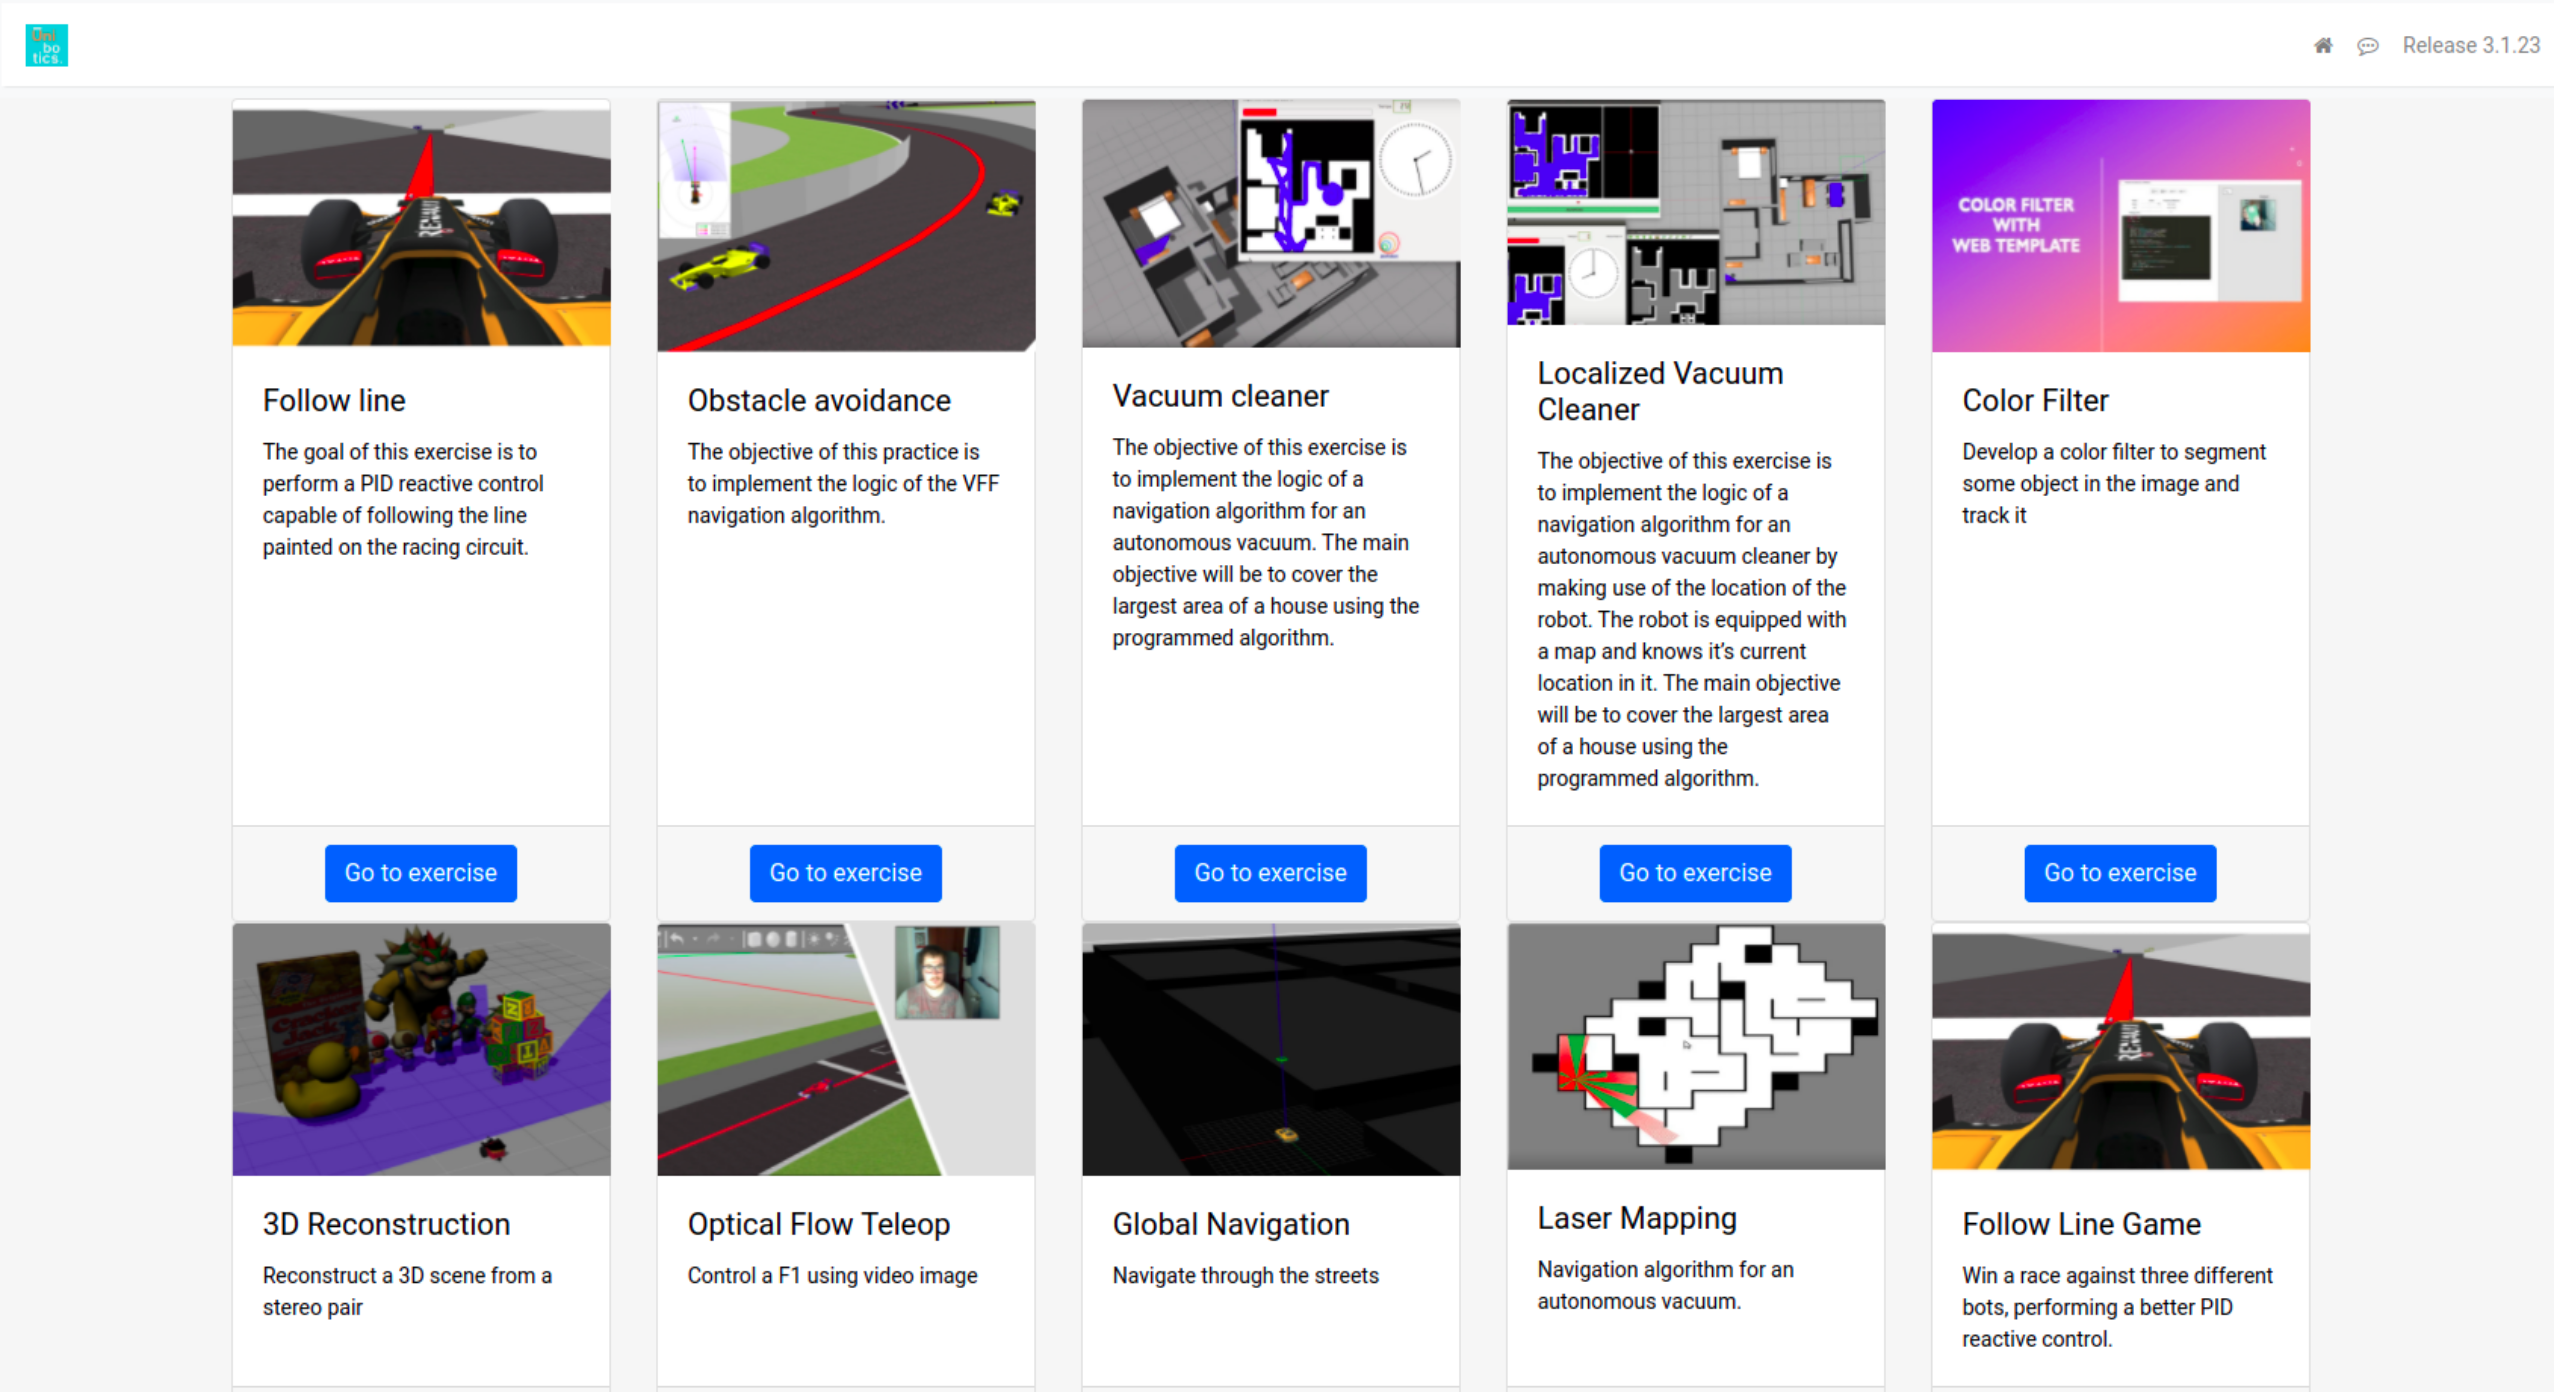
\includegraphics[width=15cm]{imagenes/unibotics-menu.png}
  \end{center}
  \caption[Unibotics (Menú)]{Unibotics (Menú)}
  \label{fig:menu-unibotics}
\end{figure}






\chapter{Objetivos y Metodología de Trabajo}
\label{cap:capitulo2}

Una vez descritos en el primer capítulo la motivación y el marco en el que se encuadra este TFG (el contexto de la robotica, la Inteligencia Artificial y las plataformas educativas), en este segundo capítulo fijamos los objetivos concretos que nos hemos planteado para este proyecto.\\

% -- SECCION OBJETIVOS
% ----------------------
\section{Objetivos}
\label{sec:objetivos}

La importancia de los robots de servicio ha ido aumentando en los últimos años, sobre todo en campos como la salud y el entretenimiento. Con este proyecto se pretende enseñar a realizar una tarea muy común en este sector: \textit{seguir a un objetivo}.\\

El objetivo principal de este TFG es desarrollar dos ejercicios educativos en Robotics Academy para programar un robot que realice la tarea de seguir a una persona. Estos ejercicios, una vez superen ciertos tests de calidad, se incorporarán a la plataforma Unibotics. Un ejercicio consistirá en programar un robot TurtleBot2 simulado para realizar dicha tarea en un hospital, y el otro, usando el robot real. Con ello, conseguiremos fomentar la participación del alumnado o usuario con dos ejercicios donde tendrán que poner en práctica lo aprendido tanto en una simulación como en el mundo real. Para lograr esta meta, se han marcado estos subobjetivos:

\begin{enumerate}
	\item Crear soporte simulado del robot TurtleBot2 en ROS2 Foxy. La última versión simulada del TurtleBot2 se encuentra en ROS Noetic distribuido por The Construct\footnote{\textbf{Turtlebot2 (Noetic):} \url{https://bitbucket.org/theconstructcore/turtlebot/src/noetic/}}. Profundizaremos más en el capítulo \ref{cap:capitulo4}
	\item Entender la infraestructura de Robotics Academy y aprender a desarrollar un nuevo ejercicio, diseñando su plantilla web (frontend) y sus propios ficheros específicos (exercise.py, interfaces con ROS, y módulos HAL y GUI). Veremos más en el capítulo \ref{cap:capitulo5}
	\item Diseñar un escenario en el simulador para el ejercicio Sigue-Persona simulado (incorporando un hospital de un repositorio externo de AWS) y programando un \textit{plugin} \footnote{\textbf{plugin}: Complemento que añade una funcionalidad extra o mejora a un programa} que permita controlar a una persona simulada desde el navegador web.
	\item Controlar el robot real a través de un contenedor Docker. Un robot que se conecta a un portatil abre muchos dispositivos (/dev) que necesitan ser mapeados para ser utilizados desde dentro del contenedor.
	\item Diseñar una solución de referencia para cada ejercicio. De este modo demostramos la posibilidad de usar el nuevo ejercicio como recurso educativo para futuros cursos académicos en el grado en Ingeniería de Robótica Software y en otros ámbitos. Además, enseñamos un posible modo de resolver el problema Sigue-Persona en el capítulo \ref{cap:capitulo6}
\end{enumerate}



% -- SECCION METODOLOGÍA
% ------------------------
\section{Metodología}
\label{sec:metodologia}
El TFG comenzó en octubre de 2021 y finalizó en mayo de 2022. Durante estos meses se ha seguido el siguiente protocolo:

\begin{itemize}
	\item Reuniones semanales con el tutor de TFG para comentar los avances y recibir retroalimentación. De esta manera abordábamos varios problemas buscando otras soluciones.
	\item Se ha usado la plataforma Slack\footnote{\textbf{Slack:} \url{https://slack.com/intl/es-es/}} para estar en comunicación con el equipo de desarolladores de Robotics Academy y de Unibotics.
	\item Anotaciones semanales en un \textit{Blog}\footnote{\textbf{Weblog}: \url{https://roboticslaburjc.github.io/2021-tfg-carlos-caminero/}} de las pruebas realizadas o logros conseguidos. De esta manera mostramos el progreso del trabajo desde sus comienzos.
	\item Todas las pruebas realizadas así como el código fuente del proyecto se han ido subiendo, a lo largo de estos meses, en un repositorio en Github habilitado dentro de la cuenta de \textit{Robotics Lab URJC}\footnote{\textbf{Repositorio TFG:} \url{https://github.com/RoboticsLabURJC/2021-tfg-carlos-caminero}}
\end{itemize}


% -- SECCIÓN PLAN DE TRABAJO
% ----------------------------
\section{Plan de Trabajo}
\label{sec:plan_trabajo}
A lo largo de estos meses, la planificación del TFG ha sido la siguiente:

\begin{enumerate}
	\item Etapa de Entrenamiento. Se correspondió al primer mes donde se empezó a probar distintas tecnologías para elegir correctamente el tema a desarrollar: Behavior Trees, Groot, aplicaciones en ROS2, ROS Bridge, etc.
	\item Inicio del TFG. Una vez conocido el tema, comenzamos a organizar el proyecto, preparando el entorno ROS, programando un \textit{plugin} para mover una persona simulada y migrando el TurtleBot2 a ROS2 Foxy. También fue necesario aprender varias herramientas y tecnologías para su elaboración:
	\begin{itemize}
		\item Aprender a construir imágenes Docker personalizadas.
		\item Profundizar en Xacro y \textit{plugins} a través de la página oficial de ROS2 Foxy\footnote{\textbf{Ros Foxy doc}: \url{https://docs.ros.org/en/foxy/}}.
		\item Para profundizar en HTML, CSS y JavaScript se ha consultado el curso del profesor \textit{Juan González Gomez} de la asignatura de Construcción de Servicios y Aplicaciones Audiovisuales en Internet (CSAAI) \cite{CSAAI}.
	\end{itemize}
	\item Programación de la infraestructura de los ejercicios.
	\begin{itemize}
		\item Primero se empezó con el ejercicio Sigue-Persona simulado: se implementó el escenario del simulador Gazebo y se programó un \textit{plugin} para mover a una persona simulada con el teclado. Después desarrollamos la plantilla web para la programación del ejercicio y la integramos en un contenedor Docker, usando como referencia otros ejercicios de Robotics Academy como por ejemplo \textit{Color Filter} \footnote{\textbf{Color filter (foxy github):} \url{https://github.com/JdeRobot/RoboticsAcademy/tree/foxy/exercises/static/exercises/color_filter/web-template}} o \textit{Follow Line} \footnote{\textbf{Follow Line (noetic github):} \url{https://github.com/JdeRobot/RoboticsAcademy/tree/master/exercises/static/exercises/follow_line/web-template}}, y, adaptándolo a ROS2.
		\item De manera similar, hicimos lo mismo con el ejercicio Sigue-Persona Real. Al tener que usar un robot real, contaba con todo el hardware necesario tanto por parte de mi tutor (todo tipo de cámaras para hacer pruebas) como por parte del laboratorio de Robótica de la ETSIT (el robot TurtleBot2, y los láseres RPLIDAR).
	\end{itemize}
	\item Programación de una solución de referencia para cada ejercicio Sigue-Persona de Robotics Academy.
	\item Memoria de Trabajo Fin de Grado. La redacción de la presente memoria se realizó durante los últimos 4 meses del curso. 
\end{enumerate}




\chapter{Herramientas utilizadas}
\label{cap:capitulo3}

En este capítulo se describen las herramientas y tecnologías utilizadas para la elaboración de los 2 ejercicios de Unibotics. Su desarrollo ha abarcado varios campos: programación del comportamiento autónomo del Robot mediante ROS 2, desarrollo de la imagen docker RADI versión 4 de Unibotics, uso hardware específico para el robot Turtlebot 2 real, etc.\\

\section{ROS (Robot Operating System)}
\label{sec:ros}
ROS (Robot Operating System) es un middleware que ayuda a la programación de robots a través de varias librerías y herramientas desarrolladas por la comunidad de software libre. Entre las ayudas que proporciona este framework están la abstracción del hardware, controladores de dispositivos y de herramientas de visualización entre otros.\\

La primera versión de ROS salió en 2010 (ROS Box Turtle) y a partir de ahí han ido surgiendo nuevas versiones siendo la actual y estable ROS Noetic.\\

El funcionamiento de ROS se basa en un sistema centralizado donde un nodo principal se encarga del intercambio de información entre otros nodos del que forma la aplicación, los cuales se comportan como publicadores o suscriptores, permitiendo así, ejecutar en paralelo varios procesos que se dedican a subtareas específicas del robot. De esta forma, por ejemplo, se puede tener un nodo encargado de la recogida de datos de la cámara y otro que comande velocidades dependiendo del resultado del procesamiento que se ha obtenido del nodo de visualización.\\

\begin{figure} [H]
  \begin{center}
    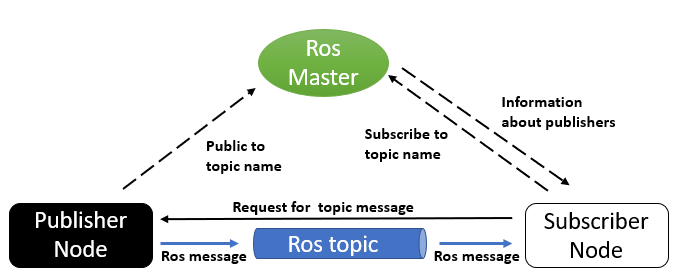
\includegraphics[width=15cm]{imagenes/ros_master_communication.png}
  \end{center}
  \caption{Comunicación del nodo Master con los nodos Intermedios (ROS)}
  \label{fig:ros_master_comunicación}
\end{figure}\

De manera paralela, ha ido surgiendo ROS 2 que es una versión en auge que incorpora nuevas características y novedades en cuanto a su uso. Al igual que en ROS se basa en publicadores y suscriptores, sin embargo, no usa un nodo maestro, y posee mecanismos de seguridad para asegurar la autenticación de los nodos y la integración de los mensajes. La versión mas reciente y estable es \textbf{ROS Foxy}. Es la distribución usada en este proyecto.\\

Los lenguajes de programación que soporta tanto ROS como ROS 2 son C++ y Python.\\

\section{URDF}
\label{sec:urdf}

\textbf{URDF (United Robotics Description Format)} es un lenguaje de marcado para describir robots (eslabones, uniones, jerarquías, modelo visual, modelo de collisión, modelo inercial, controladores, etc) que usa la gramática de XML. Se utiliza tanto para robots reales como simulados.\\

La sintaxis sigue la siguiente \textbf{regla}: El robot se divide en su mayoría en eslabones (links) y uniones entre eslabones (joints), de manera que se forma un árbol jerárquico desde un eslabón principal (root) hasta los eslabones terminales.\\

Para definir un link hay que proporcionarle su modelo visual (<visual>), su modelo de colisión (<collision>) y su modelo inercial (<inertial>). Después se define el joint que une el eslabón que hemos definido con otro mediante una jerarquía de padres e hijos.\\

\begin{code}[H]
\begin{lstlisting}[language=XML]
<?xml version="1.0"?>
<robot name="simple_cube">
	<link name="base_link">
		<visual>
			<origin xyz="0 0 0"/>
			<geometry>
				<box size="1.0 1.0 1.0"/>
			</geometry>
		</visual>
		<collision>
			<origin xyz="0 0 0"/>
			<geometry>
				<box size="1.0 1.0 1.0"/>
			</geometry>
		</collosion>
		<inertial>
			<origin xyz="0 0 0" /> 
			<mass value="1.0" />
			<inertia  ixx="1.0" ixy="0.0"  ixz="0.0"  iyy="1.0"  iyz="0.0"  izz="1.0"/>
		</inertial>
	</link>
</robot>
\end{lstlisting}
\caption[Ejemplo de código URDF: Definición de un cubo]{Ejemplo de código URDF: Definición de un cubo}
\label{cod:codigo_urdf}
\end{code}

\section{XACRO}
\label{sec:xacro}

XACRO (TODO)

\section{C++}
\label{sec:c++}

C++ es un lenguaje de programación diseñado en 1979 de Bjarne Stroustrup. Deriva del lenguaje C, y destaca principalmente porque incorpora el paradigma de la Programación Orientada a Objetos (POO). Además, incorpora una gran cantidad de nuevas librerías para facilitar la programación entre ellas las librerías estandar y STL (Standard Template Library).\\

Muchos paquetes de ROS se programan con C++ debido a la gran cantidad de posibilidades que presenta este lenguaje para desarrollar Plugins, Behavior Trees, Máquinas de Estado, etc.\\

\begin{code}[H]
\begin{lstlisting}[language=C++]
#include <iostream>

int main(int argc, char ** argv)
{
	std::cout << "Hello World!\n";
	return 0;
}
\end{lstlisting}
\caption[Hola mundo en C++]{Hola mundo en C++}
\label{cod:holamundo_cplusplus}
\end{code}


\section{Python}
\label{sec:python}

Python es un lenguaje de programación interpretado que destaca por su legibilidad, facilidad y soportabilidad a la programación Orientada a Objetos. Posee características particulares que lo diferencian de otros lenguajes de programación como puede ser el uso estricto de indentación en bloques de código.\\

La infraestructura de Unibotics y de Robotics Academy están programadas en Python

\begin{code}[H]
\begin{lstlisting}[language=Python]
print("Hola mundo")
\end{lstlisting}
\caption[Hola mundo en Python]{Hola mundo en Python}
\label{cod:holamundo_python}
\end{code}

\section{Javascript}
\label{sec:javascript}

Javascript es un lenguaje de programación interpretado que destaca por ser utilizado en el lado del cliente, en el Frontend de una página web que lee el navegador. Con Javascript podemos crear páginas web dinámicas a través de la definición de eventos que provocan resultados en el Backend (si tiene) o en la propia estructura HTML. Javascript puede usarse para más cosas: Websockets, Canvas, Animaciones, etc...\\

En las plantillas web de Robotics Academy se usa Javascript para comunicar los eventos del exercise.html con exercise.py

\section{HTML}
\label{sec:html}

HTML (TODO)

\section{CSS}
\label{sec:css}

CSS (TODO)

\section{Docker}
\label{sec:docker}

Docker (TODO)


\chapter{Migración de Turtlebot 2 de ROS Noetic a ROS Foxy}
\label{cap:capitulo4}

(TODO)

\chapter{Ejercicio Sigue Personas simulado en Robotics Academy}
\label{cap:capitulo5}

En este capítulo se presenta la elaboración del ejercicio Follow Person para Robotics Academy empezando desde el desarrollo interno de la infraestructura del ejercicio hasta una solución óptima de referencia que realice la tarea de seguir a una persona.



% -- SECCION ENTORNO GAZEBO
% ---------------------------
\section{Entorno simulado de un hospital}
\label{sec:hospital_gazebo}

La primera tarea fue integrar un entorno para Gazebo en el cual el robot Turtlebot2 tendría que enfrentarse. El entorno candidato que elegimos fue un \textbf{Hospital} debido a las siguientes ventajas:

\begin{enumerate}
	\item El robot se enfrenta a un entorno complejo (paredes, obstáculos, varias personas).
	\item La tarea Sigue Personas tendría lugar en un entorno en el cuál tiene sentido verlo en el mundo real. Los Robots en el ámbito de la salud están en continua integración.
\end{enumerate}

De modo que incorporamos el siguiente mundo de Gazebo que proporciona AWS (Amazon Web Service) en uno de sus repositorios de Github \footnote{\url{https://github.com/aws-robotics/aws-robomaker-hospital-world}}:

\begin{figure} [H]
  \begin{center}
    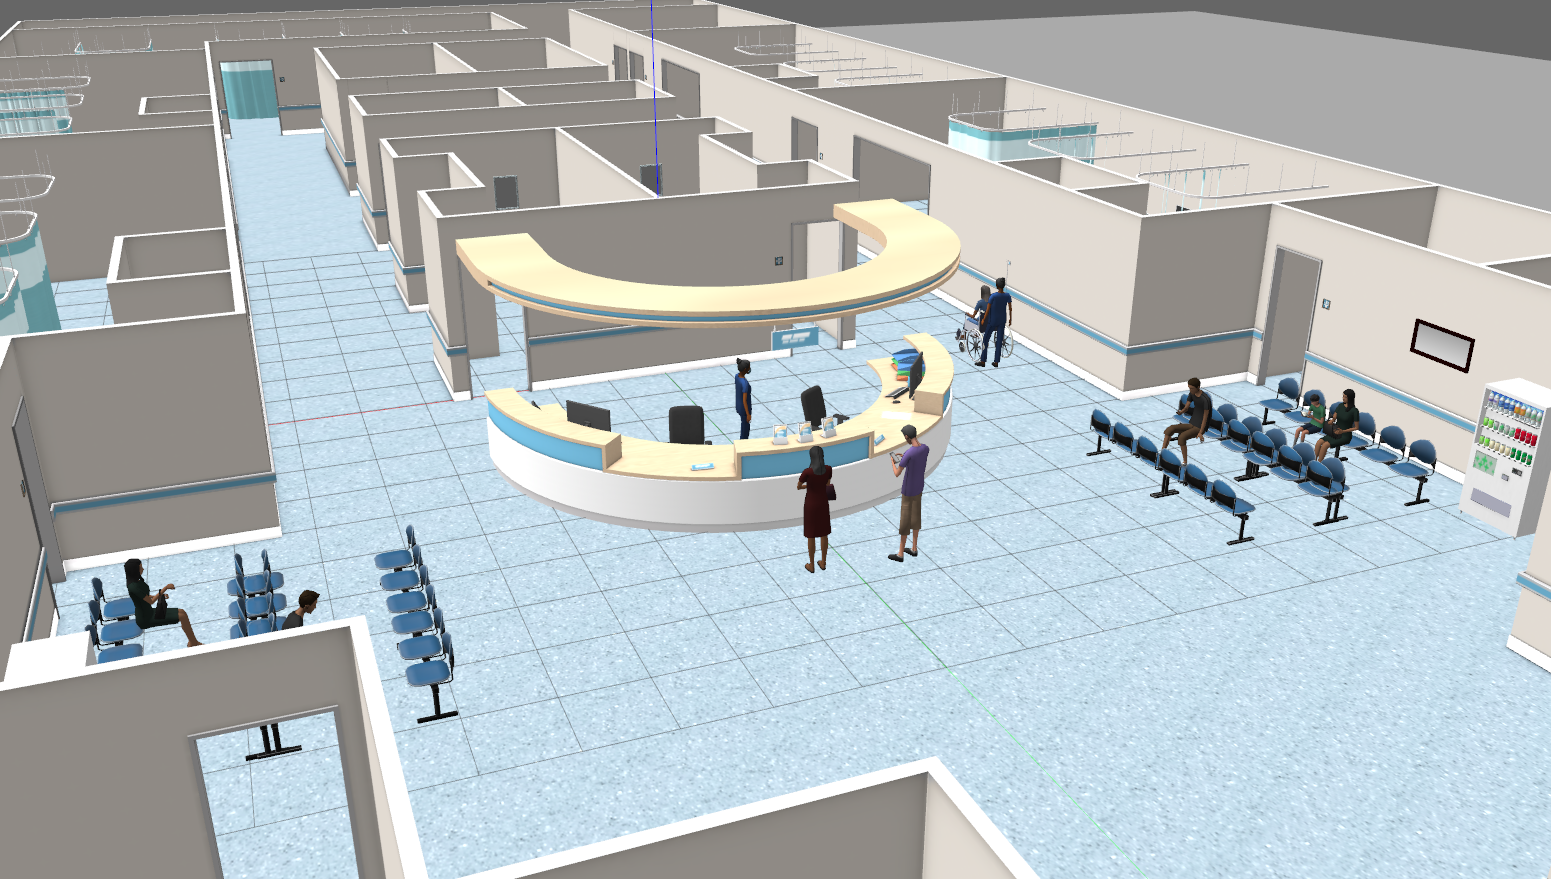
\includegraphics[width=10cm]{imagenes/hospital_world.png}
  \end{center}
  \caption[Hospital de AWS en Gazebo]{Hospital de AWS en Gazebo}
  \label{fig:hospital_gazebo}
\end{figure}

El repositorio proporcionaba varios ficheros \textbf{.world} con distintas versiones del Hospital: solo planta baja, una planta y dos plantas. Elegimos por comodidad la primera.\\

El siguiente paso era integrar una persona que pudiera desplazarse por el entorno.



% -- SECCION TELEOPERADOR
% -------------------------
\section{Teleoperador}
\label{sec:teleoperador}

El objetivo final es que el usuario que use la plantilla web pueda mover manualmente una persona del Hospital para que el robot pueda seguirla. Para ello teníamos que desarrollar un teleoperador.\\

El primer punto de partida era integrar una persona en el nuevo entorno simulado, por lo que accedimos a este repositorio \footnote{\url{https://github.com/osrf/gazebo_models}} que incorpora una librería de modelos para Gazebo e insertamos en el repositorio de Robotics Academy de terceros \textbf{Custom Robots} el modelo \textbf{\textit{person standing}}

\begin{figure} [H]
  \begin{center}
    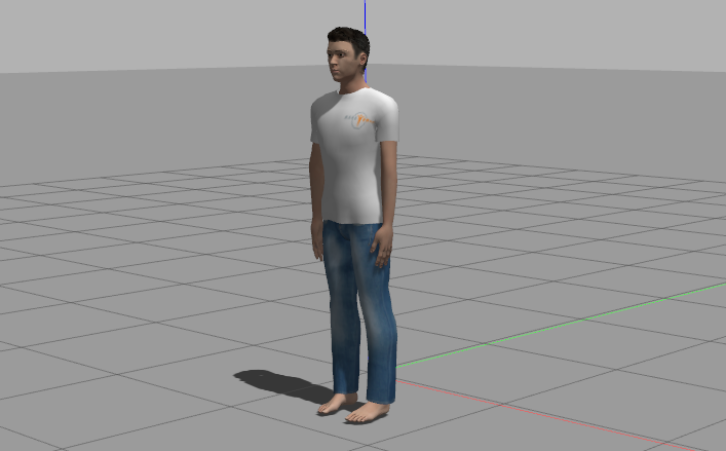
\includegraphics[width=10cm]{imagenes/person_model.png}
  \end{center}
  \caption[Persona simulada en Gazebo]{Persona simulada en Gazebo}
  \label{fig:persona_gazebo}
\end{figure}

Ahora bien, el modelo es estático, carece de capacidad de desplazamiento, por lo que fue necesario desarrollar un plugin para Gazebo que permitiera ser controlado o que pueda desplazarse a través de una ruta que eligiera el programador. De modo que en el mismo paquete donde tenía los ficheros de lanzamiento del hospital diseñe el plugin (escrito en C++) al que denominé \textbf{libpersonplugin.so} para incorporarlo en el fichero \textbf{.sdf} (similar a URDF) de la persona. En este enlace podréis ver el \textbf{código fuente}\footnote{\url{https://github.com/JdeRobot/CustomRobots/blob/foxy-devel/amazon_hospital/hospital_world/src/person.cpp}}\\

El plugin requiere \textbf{2 funcionalidades}:
\begin{enumerate}
	\item \textbf{Comunicación remota} para el control manual. La intención es que el usuario se comunique con el modelo simulado, por lo tanto diseñé un \textbf{socket} de comunicaciones para dicha tarea.
	\item \textbf{Establecimiento de una ruta} por defecto y capacidad de incorporar nuevas rutas. Esta última funcionalidad no es necesaria para el ejercicio, además de que puede suponer cierta molestia al usuario, pero no se descarta su utilidad para un futuro.
\end{enumerate}


% -- SUBSECCION COMUNICACION REMOTA
% ----------------------------------
\subsection{Comunicación remota}
\label{subsec:comunicacion_remota}

En el propio fichero \textbf{person.cpp} creé 2 hilos (threads). Uno actuaría como servidor de un socket de comunicaciones que usaría el protocolo de transporte \textbf{UDP} (No esta orientado a la conexión y es más rápido). Dentro del socket implementé un protocolo de comunicación que entendierá el servidor, el cual sería únicamente receptor de los mensajes del cliente. Los mensajes que puede recibir son:

\begin{itemize}
	\item \textbf{``UVF"} (User Velocity Forward). El modelo se mueve hacia delante.
	\item \textbf{``UVB"} (User Velocity Backward). El modelo se mueva hacia atrás.
	\item \textbf{``UAR"} (User Angular Right). El modelo gira hacia la derecha.
	\item \textbf{``UAL"} (User Angular Left). El modelo gira hacia la izquiera.
	\item \textbf{``US-"} (User Stop). El modelo se detiene.
	\item \textbf{``A--"} (Autonomous). El modelo pasa a modo autónomo. Sigue la ruta establecida (actualmente desactivada).
\end{itemize}

Pero ¿dónde entra en juego el cliente? El fichero \textbf{exercise.py} incorpora un socket de comunicación UDP que se conecta al servidor del plugin a través del puerto 36677. Además, el \textbf{exercise.py} es el servidor de un WebSocket en comunicación con la plantilla web. Cuando el usuario haga click en el botón ``Teleoperate", el fichero de eventos de Javascript podrá enviar a través de un Websocket, que usa el puerto 1905, las teclas pulsadas para que el exercise.py se lo retransmita al plugin. Al iguál que en la comunicación \textbf{plugin-exercise.py}, implementé un protocolo de comunicación para \textbf{exercise.py-exercise.html}. Los mensajes que puede recibir son:

\begin{itemize}
	\item \textbf{``\#teleop\_true"}. Activa la teleoperación. A partir de ese momento, el usuario puede pulsar los botones ``awsdx". Envía un mensaje \textbf{``US-"} al plugin.
	\item \textbf{``\#teleop\_false"}. Desactiva la teleoperación. Pasa a modo autónomo (si estuviera activado). Envía una mensaje \textbf{``A--"} al plugin.
	\item \textbf{``\#key\_a"}. Envía un mensaje \textbf{``UAR"} al plugin.
	\item \textbf{``\#key\_d"}. Envía un mensaje \textbf{``UAL"} al plugin.
	\item \textbf{``\#key\_w"}. Envía un mensaje \textbf{``UVF"} al plugin.
	\item \textbf{``\#key\_s"}. Envía un mensaje \textbf{``UVB"} al plugin.
	\item \textbf{``\#key\_x"}. Envía un mensaje \textbf{``US-"} al plugin.
\end{itemize}

A continuación podemos ver un esquema que resuma la comunicación existente entre el exercise.html (incorpora el fichero ws\_code.js) con el plugin:

\begin{figure} [H]
  \begin{center}
    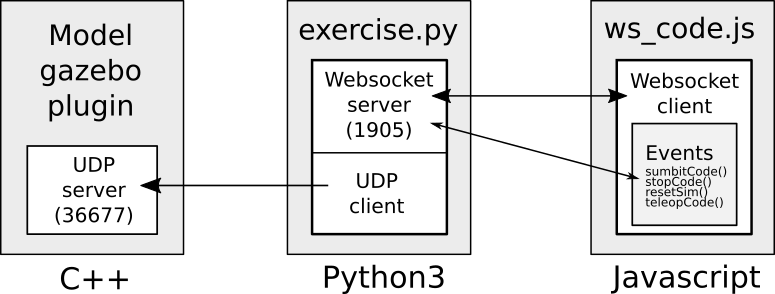
\includegraphics[width=15cm]{imagenes/comunicacion-teleoperador.png}
  \end{center}
  \caption[Comunicación del teleoperador]{Comunicación del teleoperador}
  \label{fig:comunicacion_teleoperador}
\end{figure}

% -- SUBSECCION DESPLAZAMIENTO DEL MODELO
% -----------------------------------------
\subsection{Desplazamiento del modelo}
\label{subsec:desplazamiento_modelo}
(TODO)




% -- SECCION HAL
% ----------------
\section{Desarrollo de la Capa de Abstracción Hardware (HAL)}
\label{sec:turtlebot2_hal_simulado}

En esta sección explicaremos el desarrollo de la Capa de Abstracción Hardware (HAL) que incluímos en este ejercicio, además de algunos nuevos cambios para su adaptación a ROS2.\\

Todos los ejercicios de Robotics Academy comparten una estructura muy similar. Tienen un fichero llamado \textbf{exercise.py} que se comunica tanto con el \textbf{navegador} como con los demás ficheros de su directorio. Partiendo de dicha ruta relativa, hay un directorio denominado \textbf{interfaces} donde encontramos ficheros python que actuan a modo de plantilla para comunicarse con nodos de ROS dedicados. En todos hubo que hacer algunas modificaciones debido al cambio de ROS 1 a ROS 2 (modo de creación de los nodos, publicadores y suscriptores). Como ficheros \textit{interfaces} tenemos la cámara, el láser, los motores, la odometría, y la detección mediante SSD entre otros.\\

La gran novedad se encuentra en el fichero \textbf{ssd\_detection.py}. En él definimos la clase \textbf{BoundingBox} y la clase \textbf{NeuralNetwork}:\\

La clase \textbf{BoundingBox} tiene los siguientes atributos:
\begin{itemize}
	\item \textbf{id}: Es un entero que identifica un tipo de objeto.
	\item \textbf{class\_id}: Es una cadena de texto que identifica un tipo de objeto. Con el atributo \textbf{id} forman una pareja que se puede observar en un fichero que importamos llamado \textbf{coco\_labels.py} donde se registran todos los tipos de objetos que puede detectar la red neuronal.
\begin{lstlisting}
LABEL_MAP = {
    0: "unlabeled",
    1: "person",
    2: "bicycle",
    3: "car",
    4: "motorcycle",
    5: "airplane",
    6: "bus",
    7: "train",
    8: "truck",
...
}
\end{lstlisting}
	\item \textbf{score}: Es un número en coma flotante que va de 0 a 1 que indica la \textbf{probabilidad} de que el objeto detectado coincida con la clasificación de la red neuronal. Su elección se debe a que ha sido seleccionado como el objeto con mayor porcentaje de la lista \textbf{LABEL\_MAP}
	\item \textbf{xmin} e \textbf{ymin}: Indican las coordenadas (x, y) del extremo superior izquierdo del Bounding Box.
	\item \textbf{xmax} e \textbf{ymax}: Indican las coordenadas (x, y) del extremo inferior derecho del Bounding Box.
\end{itemize}

En la clase \textbf{NeuralNetwork}, encapsulamos la importación de los ficheros que definen la red neuronal (SSD): \textbf{ssd\_inception\_v2\_coco.pb} y \textbf{ssd\_inception\_v2\_coco.pbtxt}. La creación de la red neuronal se usará con OpenCv usando la función \textbf{cv2.dnn.readNetFromTensorFlow(model, config)} al que se le pasa como argumentos la ruta a los 2 ficheros citados anteriormente. Creamos un método llamado \textbf{detect(self, img)} que se encarga de llamar internamente al modelo para realizar una detección sobre una imagen.\\

Una vez creado los ficheros \textbf{interfaces} crearemos la API de HAL en el fichero \textbf{hal.py}. Nuestro módulo (que usará el usuario) tendrá las siguientes funciones:
\begin{itemize}
	\item \textbf{setV(velocity)}. Nos permite usar velocidades lineales. Usa la interfaz \textbf{motors} que publica sobre el topic \textbf{/cmd\_vel}
	\item \textbf{setW(velocity)}. Nos permite usar velocidades angulares (radianes). Usa también la interfaz \textbf{motors} para publicar sobre el mismo topic.
	\item \textbf{getLaserData()}. Devuelve las lecturas del láser a través de un tipo de datos llamado \textbf{LaserData} usando la interfaz \textbf{laser} que se suscribe al topic \textbf{/scan}.
	\item \textbf{getImage()}. Devuelve una imagen en formato OpenCV a través de la interfaz \textbf{camera} suscrita al topic \textbf{/depth\_camera/image\_raw}
	\item \textbf{getPose3d()}. Obtiene la posición actual del robot a través de la interfaz \textbf{pose3d} suscrita al topic \textbf{/odom}
	\item \textbf{getBoundingBoxes(img)}. Dada una imagen realiza una llamada al modelo de red neuronal para realizar una detección y devolver una lista de Bounding Boxes.  
\end{itemize}

El láser RPLIDAR 360 del fichero de configuración URDF está colocado de tal manera que el ángulo 0 apunta hacia delante del robot y en sentido anti-horario. Para una correcta lectura del láser propongo la siguiente función para colocarla en el editor de texto de la plantilla web:

\begin{code}[H]
\begin{lstlisting}
def parse_laser_data(laser_data):
    values = laser_data.values
    aux = values[90:0:-1] + values[0:1] + values[360:270:-1]
    values = []
    for i in range(len(aux)):
        dist = aux[i]
        if dist == float("inf"):
            continue
        angle = math.radians(i)
        values += [(dist, angle)]
    return values
\end{lstlisting}
\caption[Transformador de lecturas del láser]{Transformador de lecturas del láser}
\label{cod:holamundo_cplusplus}
\end{code}

Con esta función leeremos como máximo 180 lecturas láser y con valores definidos. En la figura \ref{fig:vista_planta_turtlebot2} podemos ver la nueva distribución del láser hallándose el ángulo 0 a la izquierda del robot.

\begin{figure} [H]
  \begin{center}
    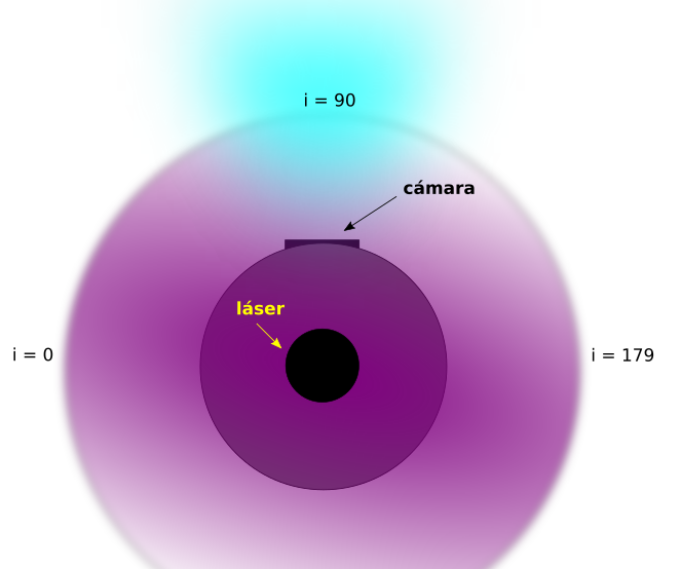
\includegraphics[width=10cm]{imagenes/vista-planta-turtlebot2.png}
  \end{center}
  \caption[Láser Turtlebot 2]{Láser Turtlebot 2}
  \label{fig:vista_planta_turtlebot2}
\end{figure}



% -- SECCION SIGUE PERSONAS
\section{Solución Sigue-Personas Simulado}
\label{sec:sigue_personas_simulado}

En esta sección explicaremos la elaboración de una solución de referencia para el problema Sigue Personas de este ejercicio en simulado. La solución la podemos dividir en 3 subobjetivos: a) detección mediante Machine Learning y seguimiento mediante un Tracker, b) desarrollo de un algoritmo de evitación de obstáculos y c) creación de una máquina de estados.


% -- SUBSECCION TRACKER
% -----------------------
\subsection{detección mediante ML y creación de un Tracker}
\label{subsec:ml_tracker}
Para detectar a la persona usaremos la función del módulo HAL llamada \textbf{getBoundingBoxes}. Esta función realiza una ejecución sobre el modelo de red neuronal para detectar todos los objetos posibles dada una \textbf{imagen} de entrada y devuelve una lista de objetos \textbf{Bounding Box} (TODO explicados en la sección anterior). Crearemos una función llamada \textbf{\textit{draw\_bounding\_box(img, bbox, color=(23, 230, 210), thickness=2)}} con la que podremos dibujar sobre la imagen un Bounding Box dado como entrada. En este caso usaremos el color verde (0, 255, 0) e iteraremos sobre todos los Bounding Boxes obtenidos (Figura \ref{fig:deteccion_ssd_sin_filtro})\\

\begin{figure} [H]
  \begin{center}
    \includegraphics[width=10cm]{imagenes/deteccion-ssd-sin-filtro.png}
  \end{center}
  \caption[Detección mediante SSD sin filtro]{Detección mediante SSD sin filtro}
  \label{fig:deteccion_ssd_sin_filtro}
\end{figure}

Sin embargo, un modelo de red neuronal genera una \textbf{puntuación} o \textbf{score} para cada objeto detectado dependiendo de su entrenamiento, por ejemplo, en una imágen donde puede aparecer una persona y una escultura humana, es probable, que la persona detectada tenga una puntuación de un 90 \% y la escultura un 70 \% debido a su parecido. Está en la labor del programador filtrar por score para desechar los \textbf{falsos positivos}. Para ello, generamos una función que llamaremos \textbf{\textit{bounding\_boxes\_by\_score(bounding\_boxes, score\_limit)}} que filtre aquellos bounding boxes que superen una puntuación límite. Debido a la naturaleza de este modelo neuronal preentrenado, las óptimas detecciones se han comprobado empíricamente que funcionan con una puntuación superior a \textbf{0.3} (el rango es de 0 a 1). Aplicando el filtro obtenemos el siguiente resultado (Figura \ref{fig:deteccion_ssd_filtro_score})\\

\begin{figure} [H]
  \begin{center}
    \includegraphics[width=10cm]{imagenes/deteccion-ssd-filtro-score.png}
  \end{center}
  \caption[Detección mediante SSD filtrando el \textbf{Score}]{Detección mediante SSD filtrando el \textbf{Score}}
  \label{fig:deteccion_ssd_filtro_score}
\end{figure}

Tal y como vemos en la figura \ref{fig:deteccion_ssd_filtro_score}, tras el filtro de \textbf{puntuación} obtenemos una imagen donde hay 3 Bounding Boxes detectados: una persona y 2 sillas. Para quedarnos solo con las personas aplicaremos un \textbf{segundo filtro}, en la cual nos fijaremos en la \textbf{clase} del Bounding Box. Recordemos que el objeto Bounding Box tenía un atributo \textbf{id} que correspondía a un número entero y un atributo \textbf{class\_id} que era la traducción de dicho número a una cadena de texto (ej: 1 - ``person", 2 - ``bicycle"). Crearemos una función llamada \textbf{\textit{bounding\_boxes\_by\_name(bounding\_boxes, name)}} al cual dada una lista de objetos detectados pasaremos como segundo parámetro de entrada el nombre de la clase que queremos filtrar (en este caso ``person"). Aplicando el filtro obtenemos una correcta detección de personas (Figura \ref{fig:deteccion_ssd_filtro_score_class}):

\begin{figure} [H]
  \begin{center}
    \includegraphics[width=10cm]{imagenes/deteccion-ssd-filtro-score-class.png}
  \end{center}
  \caption[Detección mediante SSD filtrando el \textbf{Score} y la \textbf{Clase}]{Detección mediante SSD filtrando el \textbf{Score} y la \textbf{Clase}}
  \label{fig:deteccion_ssd_filtro_score_class}
\end{figure}

Como último filtro y muy recomendable es rechazar aquellas detecciones que no superen un \textbf{área} determinado. Con este filtro, evitamos que el robot se confunda con personas que se encuentren a una distancia lejana o con un falso positivo, para ello, crearemos una función llamada \textbf{\textit{bounding\_boxes\_by\_area(bounding\_boxes, min\_area)}} al cual dada una lista de objetos detectados pasaremos como segundo parámetro de entrada el área mínima que debe filtrar.\\

El siguiente paso es crear un \textbf{Tracker} de seguimiento. Nuestro tracker se basará en la distancia de los centroides de los Bounding Boxes de un fotograma el candidato anterior. Recordemos que un Bounding Box tenía otros 4 parámetros más: xmin e ymin correspondían a las coordenadas (x,y) del extremo superior izquierdo de la caja de detección, y xmax e ymax correspondían a las coordenadas (x,y) del extremo inferior derecho. Para obtener el \textbf{centroide} aplicaremos la siguiente fórmula:\\
\begin{eqnarray*}
C_x = \frac{x_{min} + x_{max}}{2}\\
C_y = \frac{y_{min} + y_{max}}{2}\\
\end{eqnarray*}

Crearemos una clase llamada \textbf{BoundingBoxObject} que tendrá 3 atributos: El \textbf{Bounding Box} correspondiente, su \textbf{centroide} y su \textbf{área}. El área lo obtendremos de la siguiente manera: $A = (x_{max} - x_{min}) (y_{max} - y_{min})$\\

Posteriormente, creamos una clase llamada \textbf{Tracker} que nos proporcionará una capa de abstracción al usar los siguientes métodos que definiremos:
\begin{itemize}
	\item \textbf{\textit{setObjective(self, obj)}}: Establece el objetivo BoundingBoxObject de seguimiento.
	\item \textbf{\textit{getObjective(self)}}: Devuelve el objetivo BoundingBoxObject actual de seguimiento.
	\item \textbf{\textit{getObjectiveFromSet(self, objlist)}}: Dada una lista o conjunto de objetos BoundingBoxObject, devuelve el objetivo candidato que más se acerca al anterior, y lo actualiza. El candidato seleccionado será aquel cuyo centroide esté más cerca al actual, que no supere una distancia límite de diferencia(50) y que la diferencia de área entre el BoundingBoxObject anterior y el actual sea menor a 30000. Para calcular la distancia entre centroides usaremos la Distancia Euclídea:
	\begin{equation*}
	d = \sqrt{(C_{x}' - C_{x})^2 + (C_{y}' - C_{y})^2}
	\end{equation*}
\end{itemize}

En la figura \ref{fig:obtencion_centroide} podemos ver con más detalle en qué se basa esté procedimiento: comparamos cada centroide con el centroide candidato del fotograma anterior y elegiremos aquel que cumpla los requisitos descritos anteriormente.
\begin{figure} [H]
  \begin{center}
    \includegraphics[width=10cm]{imagenes/esquema-tracker.png}
  \end{center}
  \caption[Modo de obtención del centroide candidato]{Modo de obtención del centroide candidato}
  \label{fig:obtencion_centroide}
\end{figure}

Al principio del programa inicalizaremos una \textbf{instancia} de tipo Tracker, y, en cada iteración del bucle principal al método \textbf{getObjectiveFromSet(self, objlist)} para obtener un BoundingBoxObject que dibujaremos en la imagen de color rojo. El resultado será el siguiente:

\begin{figure} [H]
  \begin{center}
    \includegraphics[width=10cm]{imagenes/aplicando-tracker.png}
  \end{center}
  \caption[Usando el Tracker para no perder al objetivo]{Uso del Tracker para no perder al objetivo}
  \label{fig:uso_tracker}
\end{figure}

Como criterio de selección de la persona que seguiremos, deberá cumplir los 3 filtros indicados anteriormente, aparecer en el segundo tercio de la imagen (dividiremos la imagen en 3 y analizaremos la mitad) y ser aquel BoundingBoxObject con un área mayor que el resto.\\


% -- SUBSECCIÓN EVITAR OBSTÁCULOS
% ---------------------------------
\subsection{Algoritmo VFF}
\label{subsec:vff}

Seguir a una persona en un mundo vacío es sencillo, pero cuando el entorno presenta \textbf{obstáculos}, es importante tener ese riesgo en cuenta:

\begin{itemize}
	\item ¿Qué ocurre si la persona que seguimos gira por un pasillo a la derecha?. ¿El robot sufriría una colisión con la pared antes de girar?
	\item ¿Qué ocurre si el robot se está acercando a la pata de una mesa? ¿Y si está pasando cerca de otra persona a la que ha descartado en el proceso de Tracking?
\end{itemize}

El algoritmo de \textbf{Campo de Fuerzas Virtuales (VFF)} es el más indicado para esas situaciones. Se basa en la suma vectorial de un vector de atracción y de repulsión originando un vector resultante que indica la nueva dirección de desplazamiento. La suma vectorial estará influenciada por el valor de unos pesos llamados \textbf{alfa} y \textbf{beta} aplicados a los vectores de atraccion y repulsión respectivamente, pudiendo de esta manera, dar más valor a uno que otro.\\

El \textbf{vector de atracción} será aquel que desde el robot apuntará al objetivo. Al usar una cámara en la que no tenemos en cuenta la profundidad, estableceremos que el \textbf{módulo} del vector será siempre 2 metros. Para obtener el ángulo nos basaremos en el \textbf{Campo de Visión (FOV) horizontal} de la cámara. Al ser una cámara simulada, en su fichero urdf.xacro (tal y como vimos en el capítulo \ref{cap:capitulo4}) indicamos que FOV fuera 1.04 radianes (60 grados). Por lo tanto, 0 grados se corresponderá al centro de la imagen y los extremos a los ángulos -30 y 30. Para conocer el ángulo con el objetivo necesitaremos conocer el ancho de la imagen, y la posición de la coordenada x del centroide. La ecuación es la siguiente:\\

\begin{equation*}
\alpha = \frac{H_{FOV} \cdot C_{x}}{w} - \frac{H_{FOV}}{2}
\end{equation*}\\

Conociendo el ángulo ($\alpha$) y módulo (m) podremos obtener las \textbf{componentes x e y} del vector de atracción \textbf{A}:
\begin{eqnarray*}
A_x = m \cdot sin(\alpha)\\
A_y = m \cdot cos(\alpha)\\
\end{eqnarray*}

El \textbf{vector de repulsión} se calculará a partir de todas las lecturas del láser. Cada obstáculo presente en el rango del láser provocará un vector en sentido contrario cuyo módulo estará influenciado por una constante y será inversamente proporcional a la distancia con el obstáculo (es decir, cuanto más cerca, mayor será el módulo). Sabiendo la constante (K) y la distancia (d) de cada lectura del láser (n lecturas), la ecuación del vector de repulsión (R) es la siguiente:

\begin{eqnarray*}
R_x &=& \sum_{i=1}^n\left(\frac{K}{d_i}\right)^2 \cdot cos(\alpha)\\
R_y &=& \sum_{i=1}^n\left(\frac{-K}{d_i}\right)^2 \cdot sin(\alpha)\\
\end{eqnarray*}

En la ecuación vemos como la componente $R_y$ va en dirección contraria al desplazamiento del robot. La potencia de 2 se aplica para evitar \textbf{mínimos locales}\\

El \textbf{vector final (F) o resultante} lo obtendremos sumando las componentes de los vectores de atracción y repulsión. Ambos multiplicados por 2 constantes $\alpha$ y $\beta$ respectivamente. La ecuación queda de esta manera.

\begin{eqnarray*}
F_x &=& \alpha \cdot A_x + \beta \cdot R_x\\
F_y &=& \alpha \cdot A_y + \beta \cdot R_y\\
\end{eqnarray*}

Queda en la labor del programador ajustar empíricamente los parámetros $\alpha$ y $\beta$ dependiendo del comportamiento que desee. Si queremos darle más peso a la repulsión aumentaremos $\beta$ pero en casos extremos podríamos llegar a perder el objetivo. En cambio si queremos darle más perso a la atracción conseguiremos que evité los obstáculos sin perder al objetivo pero si está mal ajustado podríamos colisionar a causa de una escasa repulsión. En la figura \ref{fig:esquema_vff} resumimos el algoritmo VFF de manera gráfica para una mejor comprensión.\\

\begin{figure} [H]
  \begin{center}
    \includegraphics[width=10cm]{imagenes/esquema-vff.png}
  \end{center}
  \caption[Algoritmo VFF]{Algoritmo VFF}
  \label{fig:esquema_vff}
\end{figure}

En nuestra solución de referencia, aplicaremos solamente la componente $F_x$ como velocidad angular, ya que la velocidad lineal estará \textbf{basada en casos} dependiendo de la distancia al objetivo. En el siguiente apartado [\ref{subsec:maquina_estados}] lo explicaremos con más detalle.

% -- SUBSECCION MÁQUINA DE ESTADOS
% ----------------------------------
\subsection{Máquina de Estados}
\label{subsec:maquina_estados}

Como último paso de la solución, queda implementar una máquina de estados que le dé al robot la capacidad de tomar distintas acciones dependiendo del estado en el que se encuentre. En nuestro caso, hemos definido \textbf{2 estados}: Buscar-Persona y Seguir-Persona.\\

El estado \textbf{Buscar-Persona} será aquel con el que empecemos la ejecución del programa. Al principio, girará a una velocidad angular determinada mientras aplica los 3 filtros de detección sobre la imagen para detectar personas. Transitará al siguiente estado cuando el robot identifique un candidato a seguir (mayor área del BoundingBoxObject y posicionado en la franja central de la imagen).\\

En el estado \textbf{Seguir-Persona} aplicaremos el algoritmo de Tracking [\ref{subsec:ml_tracker}] y VFF [\ref{subsec:vff}]. Además, la velocidad lineal cambiará dependiendo de la distancia al objetivo. Para ello crearemos unas condiciones en las que dependiendo del área del Bounding Box aplicaremos una velocidad u otra. Cuanto más pequeño sea el área, más lejos estará nuestro objetivo. Si por algún motivo perdemos a la persona, incrementaremos un \textbf{contador de fallo} y de esta manera, en caso de no detectarla en el siguiente fotograma, nos quedaremos con el mismo valor del centroide candidato. Cuando el contador supere un límite, transitaremos al primer estado: \textbf{Buscar-Persona}.\\

El \textbf{resultado de nuestra solución} podéis verla en el siguiente enlace: \textbf{\textit{https://youtu.be/fDAU465eVxQ}}



\chapter{Soluciones de referencia}
\label{cap:capitulo6}

En este capítulo abordamos una solución de referencia para los ejercicios Sigue-Persona Simulado y Sigue-Persona Real. Con los dos ejercicios el usuario podrá poner a prueba su algoritmo. Se pretende poner en práctica la experiencia del programador robótico cuando desarrolla una aplicación robótica. El primer paso es probar su programa en una simulación (Sigue-Persona Simulado). Una vez que su solución es bastante robusta, pasa al siguiente nivel, probándolo en el mundo real (Sigue-Persona Real). El programador se dará cuenta de que es muy probable que el mismo programa en simulación no funcione exactamente igual con un robot real. Si su solución es bastante buena y robusta, solamente tendrá que ajustar algunos parámetros y tener en cuenta ciertos factores (como por ejemplo la luz ambiental o el rendimiento de CPU) y habrá logrado su objetivo.\\

\section{Solución Sigue-Persona Simulado}
\label{sec:solucion_sigue_personas_simulado}

La solución que resuelve la aplicación de \textit{Seguir a una persona} la podemos dividir en 3 subobjetivos: a) detección mediante redes neuronales y seguimiento mediante un Tracker, b) desarrollo de un algoritmo de evitación de obstáculos y c) creación de una máquina de estados.\\



% -- SUBSECCION TRACKER
% -----------------------
\subsection{Detección mediante RNA y creación de un Tracker}
\label{subsec:ml_tracker}
Para detectar a la persona usamos la función del módulo HAL llamada \textit{getBoundingBoxes}. Esta función realiza una inferencia del modelo de red neuronal para detectar todos los objetos posibles dada una imagen de entrada y devuelve una lista de objetos de cajas de detección (explicados en la Sección [\ref{sec:plantilla_python}]). Crearemos una función llamada \textit{draw\_bounding\_box(img, bbox, color=(23, 230, 210), thickness=2)} con la que podremos dibujar sobre la imagen una caja de detección dada como entrada. En este caso usaremos el color verde (0, 255, 0) e iteraremos sobre todos las cajas de detección obtenidas (Figura \ref{fig:deteccion_ssd_sin_filtro})\\

\begin{figure} [H]
  \begin{center}
    \includegraphics[width=10cm]{imagenes/cap6/deteccion-ssd-sin-filtro.png}
  \end{center}
  \caption[Detección mediante SSD sin filtro]{Detección mediante SSD sin filtro}
  \label{fig:deteccion_ssd_sin_filtro}
\end{figure}\

Un modelo de red neuronal genera una puntuación o \textit{score} para cada objeto detectado dependiendo de su entrenamiento. Por ejemplo, en una imagen donde puede aparecer una persona y una escultura humana, es probable, que la persona detectada tenga una puntuación de un 90 \% y la escultura un 70 \% debido a su parecido. Está en la labor del programador filtrar por \textit{score} para desechar los falsos positivos. Para ello, generamos una función que llamaremos \textit{bounding\_boxes\_by\_score(bounding\_boxes, score\_limit)} que filtre aquellas cajas de detección que superen una puntuación límite. Debido a la naturaleza de este modelo neuronal preentrenado, las óptimas detecciones se han comprobado empíricamente que funcionan con una puntuación superior a 0.3 (el rango va de 0 a 1). Aplicando el filtro obtenemos el siguiente resultado (Figura \ref{fig:deteccion_ssd_filtro_score})\\

\begin{figure} [H]
  \begin{center}
    \includegraphics[width=10cm]{imagenes/cap6/deteccion-ssd-filtro-score.png}
  \end{center}
  \caption[Detección mediante SSD filtrando la puntuación de clasificación]{Detección mediante SSD filtrando la puntuación de clasificación}
  \label{fig:deteccion_ssd_filtro_score}
\end{figure}\

Tal y como vemos en la Figura \ref{fig:deteccion_ssd_filtro_score}, tras el filtro de puntuación obtenemos una imagen donde hay tres cajas de detección detectadas: una persona y dos sillas. Para quedarnos solo con las personas aplicaremos un \textit{segundo filtro}, en la cual nos fijaremos en la clase del Bounding Box. Recordemos que el objeto Bounding Box tenía un atributo \textit{id} que correspondía a un número entero y un atributo \textit{class\_id} que era la traducción de dicho número a una cadena de texto (ej: 1 - ``person", 2 - ``bicycle"). Crearemos una función llamada \textit{bounding\_boxes\_by\_name(bounding\_boxes, name)} al cual dada una lista de objetos detectados pasaremos como segundo parámetro de entrada el nombre de la clase que queremos filtrar (en este caso ``person"). Aplicando el filtro obtenemos una correcta detección de personas (Figura \ref{fig:deteccion_ssd_filtro_score_class}):\\

\begin{figure} [H]
  \begin{center}
    \includegraphics[width=10cm]{imagenes/cap6/deteccion-ssd-filtro-score-class.png}
  \end{center}
  \caption[Detección mediante SSD filtrando la puntuación y la clase]{Detección mediante SSD filtrando la puntuación y la clase}
  \label{fig:deteccion_ssd_filtro_score_class}
\end{figure}

Como último filtro y muy recomendable, debemos rechazar aquellas detecciones que no superen un \textit{área} determinado. Con este filtro, evitamos que el robot se confunda con personas que se encuentren a una distancia lejana o con un falso positivo. Para ello, crearemos una función llamada \textit{bounding\_boxes\_by\_area(bounding\_boxes, min\_area)} al cual dada una lista de objetos detectados pasaremos como segundo parámetro de entrada el área mínimo que debe filtrar.\\

El siguiente paso es crear un \textit{Tracker} de seguimiento. Nuestro \textit{tracker} se basa en la distancia de los centroides de las cajas de detección del fotograma actual con el candidato del fotograma anterior. Recordemos que una caja de detección tenía otros 4 parámetros más: $x_{min}$ e $y_{min}$ correspondían a las coordenadas (x,y) del extremo superior izquierdo de la caja de detección, y $x_{max}$ e $y_{max}$ correspondían a las coordenadas (x,y) del extremo inferior derecho. Para obtener el centroide aplicamos la siguiente fórmula:\\
\begin{eqnarray*}
C_x = \frac{x_{min} + x_{max}}{2}\\
C_y = \frac{y_{min} + y_{max}}{2}\\
\end{eqnarray*}

Creamos una clase llamada \textit{BoundingBoxObject} que tiene 3 atributos: La caja de detección correspondiente, su centroide y su área. El área lo obtenemos de la siguiente manera: $A = (x_{max} - x_{min}) (y_{max} - y_{min})$.\\

Posteriormente, creamos una clase llamada \textit{Tracker} que proporcionará una capa de abstracción al usar los siguientes métodos que definimos:

\begin{itemize}
	\item \textbf{setObjective(self, obj)}: Establece el objetivo BoundingBoxObject de seguimiento.
	\item \textbf{getObjective(self)}: Devuelve el objetivo \textit{BoundingBoxObject} actual de seguimiento.
	\item \textbf{getObjectiveFromSet(self, objlist)}: Dada una lista o conjunto de objetos \textit{BoundingBoxObject}, devuelve el objetivo candidato que más se acerca al anterior, y lo actualiza. El candidato seleccionado será aquel cuyo centroide esté más cerca del actual, no supere una distancia límite(50) con él, y que la diferencia de área entre el \textit{BoundingBoxObject} anterior y el actual sea menor a 30000. Para calcular la distancia entre centroides usaremos la Distancia Euclídea:
	\begin{equation*}
	d = \sqrt{(C_{x}' - C_{x})^2 + (C_{y}' - C_{y})^2}
	\end{equation*}
\end{itemize}\

En la Figura \ref{fig:obtencion_centroide} se puede ver con más detalle en qué se basa este procedimiento: se compara cada centroide con el centroide candidato del fotograma anterior y se elige aquel que cumpla los requisitos descritos anteriormente.\\

\begin{figure} [H]
  \begin{center}
    \includegraphics[width=10cm]{imagenes/cap6/esquema-tracker.png}
  \end{center}
  \caption[Modo de obtención del centroide candidato]{Modo de obtención del centroide candidato}
  \label{fig:obtencion_centroide}
\end{figure}\

Al principio del programa inicializamos una instancia de tipo Tracker, y, en cada iteración del bucle principal llamamos al método \textit{getObjectiveFromSet(self, objlist)} para obtener un \textit{BoundingBoxObject} que dibujamos en la imagen de color rojo. El resultado queda de la siguiente manera:\\

\begin{figure} [H]
  \begin{center}
    \includegraphics[width=10cm]{imagenes/cap6/aplicando-tracker.png}
  \end{center}
  \caption[Usando el Tracker para no perder al objetivo]{Uso del Tracker para no perder al objetivo}
  \label{fig:uso_tracker}
\end{figure}\

Como criterio de selección de la persona a la que seguiremos, deberá cumplir los 3 filtros indicados anteriormente, aparecer en el segundo tercio de la imagen (dividiremos la imagen en 3 y analizaremos la mitad) y ser aquel \textit{BoundingBoxObject} con un área mayor que el resto.\\


% -- SUBSECCIÓN EVITAR OBSTÁCULOS
% ---------------------------------
\subsection{Algoritmo de navegación VFF}
\label{subsec:vff}

Seguir a una persona en un mundo vacío es sencillo, pero cuando el entorno presenta obstáculos, es importante tener ese riesgo en cuenta:

\begin{itemize}
	\item ¿Qué ocurre si la persona que seguimos gira por un pasillo a la derecha? ¿El robot sufriría una colisión con la pared antes de girar?
	\item ¿Qué ocurre si el robot se está acercando a la pata de una mesa? ¿Y si está pasando cerca de otra persona a la que ha descartado en el proceso de Tracking?
\end{itemize}

El algoritmo de \textit{Campo de Fuerzas Virtuales (VFF)} está muy indicado para esas situaciones. Se basa en la suma vectorial de un vector de atracción y de repulsión originando un vector resultante que indica la nueva dirección de desplazamiento. La suma vectorial estará influenciada por el valor de unos pesos $\alpha$ y $\beta$ aplicados a los vectores de atraccion y repulsión respectivamente, pudiendo de esta manera dar más valor a uno que otro.\\

El \textit{vector de atracción} será aquel que desde el robot apunta al objetivo. Al usar una cámara en la que no tenemos en cuenta la profundidad, establecemos que el módulo del vector será siempre 2 metros. Para obtener el ángulo nos basamos en el Campo de Visión (FOV) horizontal de la cámara. Al ser una cámara simulada, en su fichero \texttt{camera.urdf.xacro} (tal y como vimos en el capítulo \ref{cap:capitulo4}) indicamos que FOV fuera 1.04 radianes (60 grados). Por lo tanto, 0 grados se corresponderá al centro de la imagen y los extremos a los ángulos -30 y 30. Para conocer el ángulo con el objetivo necesitaremos conocer el ancho de la imagen, y la posición de la coordenada x del centroide. La ecuación es la siguiente:

\begin{equation*}
\alpha = \frac{H_{FOV} \cdot C_{x}}{w} - \frac{H_{FOV}}{2}
\end{equation*}\\

Conociendo el ángulo ($\alpha$) y módulo (m) podremos obtener las componentes x e y del vector de atracción \textit{A}:
\begin{eqnarray*}
A_x = m \cdot sin(\alpha)\\
A_y = m \cdot cos(\alpha)\\
\end{eqnarray*}

El \textit{vector de repulsión} se calculará a partir de todas las lecturas del láser. Cada obstáculo presente en el rango del láser provocará un vector en sentido contrario cuyo módulo estará influenciado por una constante y será inversamente proporcional a la distancia con el obstáculo (es decir, cuanto más cerca, mayor será el módulo). Sabiendo la constante (K) y la distancia (d) de cada lectura del láser (n lecturas), la ecuación del vector de repulsión (R) es la siguiente:

\begin{eqnarray*}
R_x &=& \sum_{i=1}^n\left(\frac{K}{d_i}\right)^2 \cdot cos(\alpha)\\
R_y &=& \sum_{i=1}^n\left(\frac{-K}{d_i}\right)^2 \cdot sin(\alpha)\\
\end{eqnarray*}

En la ecuación vemos cómo la componente $R_y$ va en dirección contraria al desplazamiento del robot. La potencia de 2 se aplica para evitar mínimos locales.\\

El \textit{vector final (F) o resultante} lo obtenemos sumando las componentes de los vectores de atracción y repulsión. Ambos multiplicados por dos constantes $\alpha$ y $\beta$ respectivamente. La ecuación queda de esta manera:

\begin{eqnarray*}
F_x &=& \alpha \cdot A_x + \beta \cdot R_x\\
F_y &=& \alpha \cdot A_y + \beta \cdot R_y\\
\end{eqnarray*}

Queda en la labor del programador ajustar empíricamente los parámetros $\alpha$ y $\beta$ dependiendo del comportamiento que desee. Si queremos darle más peso a la repulsión aumentaremos $\beta$ pero en casos extremos podríamos llegar a perder el objetivo. En cambio, si queremos darle más peso a la atracción conseguiremos que evite los obstáculos sin perder al objetivo pero si está mal ajustado podríamos colisionar a causa de una escasa repulsión. En la Figura \ref{fig:esquema_vff} resumimos el algoritmo VFF de manera gráfica para una mejor comprensión.\\

\begin{figure} [H]
  \begin{center}
    \includegraphics[width=10cm]{imagenes/cap6/esquema-vff.png}
  \end{center}
  \caption[Algoritmo VFF]{Algoritmo VFF}
  \label{fig:esquema_vff}
\end{figure}\

En nuestra solución de referencia, los valores $\alpha$ y $\beta$ que usamos fueron 0.5 y 0.05 respectivamente. Aplicamos solamente la componente $F_x$ del vector final como velocidad angular, ya que la velocidad lineal está \textit{basada en casos} dependiendo de la distancia al objetivo. Esta última depende del tamaño de la caja de detección:

\begin{itemize}
	\item Si el área es menor que 16000, el objetivo se encontrará lejos, por tanto comandaremos una velocidad lineal de 0.2 m/s.
	\item Si el área se encuentra entre 16000 y 45000, significa que el objetivo está cerca, por tanto comandaremos una velocidad lineal de 0.1 m/s.
	\item Si no se cumple ninguna de estas condiciones, el objetivo se encontrará muy cerca por tanto el robot se detendrá.
\end{itemize}\


% -- SUBSECCION MÁQUINA DE ESTADOS
% ----------------------------------
\subsection{Máquina de Estados}
\label{subsec:maquina_estados}

Como último paso de la solución, queda implementar una máquina de estados que le dé al robot la capacidad de tomar distintas acciones dependiendo del estado en el que se encuentre. En nuestro caso, hemos definido 2 estados: Buscar-Persona y Seguir-Persona.\\

El estado \textit{Buscar-Persona} será aquel con el que empecemos la ejecución del programa. Al principio, girará a una velocidad angular determinada mientras aplica los 3 filtros de detección sobre la imagen para detectar personas. Transitará al siguiente estado cuando el robot identifique un candidato a seguir (mayor área del \textit{BoundingBoxObject} y posicionado en la franja central de la imagen).\\

En el estado \textit{Seguir-Persona} aplicaremos el algoritmo de \textit{Tracking} y VFF. Además, la velocidad lineal cambiará dependiendo de la distancia al objetivo. Para ello crearemos unas condiciones en las que dependiendo del área de la caja de detección aplicaremos una velocidad u otra. Cuanto más pequeño sea el área, más lejos estará nuestro objetivo. Si por algún motivo perdemos a la persona, incrementaremos un contador de fallo y de esta manera, en caso de no detectarla en el siguiente fotograma, nos quedaremos con el mismo valor del centroide candidato. Cuando el contador supere un límite, transitaremos al primer estado: \textit{Buscar-Persona}.\\

En la Figura \ref{fig:maquina_estados} se puede ver un esquema de la Máquina de Estados Finitos (FSM) utilizada.\\

\begin{figure} [H]
  \begin{center}
    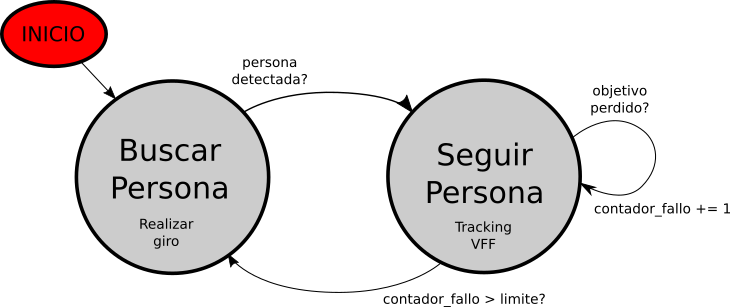
\includegraphics[width=12cm]{imagenes/cap6/maquina-estados.png}
  \end{center}
  \caption[Máquina de Estados Sigue-Persona]{Máquina de Estados Sigue-Persona}
  \label{fig:maquina_estados}
\end{figure}\


\subsection{Validación experimental}
\label{subsec:validacion_experimental_sim}

A continuación describimos la ejecución de la solución de referencia donde pusimos en prueba nuestro algoritmo:

\begin{itemize}
	\item Para probar el algoritmo de navegación VFF, colocamos dos objetos de Gazebo en frente del robot con el fin de que pudiera esquivarlos sin perder al objetivo. Primero, el robot se encontraba en el estado Buscar-Persona hasta que detecta a su objetivo en el medio de la imagen. Al transitar de estado, el robot comienza a utilizar la navegación VFF con una velocidad lineal de 0.1 m/s debido a la distancia que le separa con la persona. Al principio, debido a la repulsión del obstáculo que tiene a su derecha, el robot gira a la izquierda, pero debido al valor incremental de la componente $A_{x}$ de la fuerza del vector de atracción, el robot bordea el obstáculo. Seguidamente, realiza lo mismo con el obstáculo que tiene a su izquierda. En la Figura \ref{fig:sim_solucion_vff_test} se puede ver la prueba realizada. Después de esquivar los dos obstáculos, el robot recuperaba su estabilidad.
	
	\begin{figure} [H]
		\begin{center}
		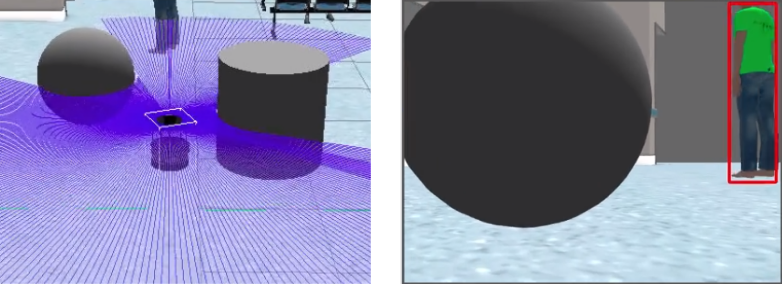
\includegraphics[width=10cm]{imagenes/cap6/sim-solution-vff-test.png}
		\end{center}
		\caption[Solución Sigue-Persona Simulado: prueba de navegación VFF]{Solución Sigue-Persona Simulado: prueba de navegación VFF}
		\label{fig:sim_solucion_vff_test}
	\end{figure}

	\item Luego, para probar el algoritmo de seguimiento (\textit{tracking}), dirigimos a la persona simulada a través del recibidor del hospital (la zona del escenario donde hay más personas) pudiendo comprobar que el robot era capaz de seguir a su objetivo sin confundirse. Poco después de comenzar el seguimiento, utilizamos a la persona simulada para alejarla lo máximo posible del robot y vimos cómo su velocidad lineal cambiaba de 0.1 m/s a 0.2 m/s. Luego pasamos cerca de una enfermera cuya caja de detección aumentaba en la parte derecha de la imagen conforme el robot se acercaba, pero no perdía a su objetivo inicial. En la Figura \ref{fig:sim_solucion_tracking_test} se puede ver la prueba que realizamos para el algoritmo de \textit{tracking} perceptivo.

	\begin{figure} [H]
		\begin{center}
		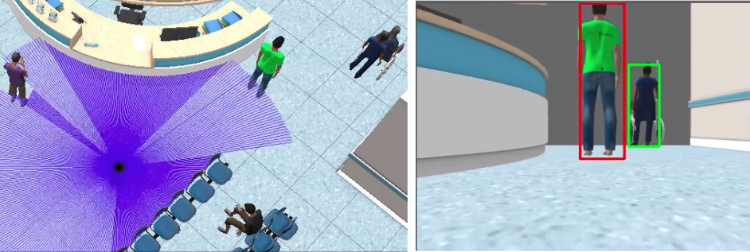
\includegraphics[width=10cm]{imagenes/cap6/sim-solution-tracking-test.png}
		\end{center}
		\caption[Solución Sigue-Persona Simulado: prueba de seguimiento]{Solución Sigue-Persona Simulado: prueba de seguimiento}
		\label{fig:sim_solucion_tracking_test}
	\end{figure}
\end{itemize}\

El vídeo de la solución que muestra todas las pruebas descritas se puede ver en el siguiente enlace: \url{https://youtu.be/fDAU465eVxQ}\\




% -- SECCION SIGUE PERSONAS REAL
% -----------------------------
\section{Solución Sigue-Persona Real}
\label{sec:solucion_sigue_personas_real}

El modo de resolver este problema es idéntico al Sigue-Persona simulado, sin embargo, el entorno sobre el que se mueve el robot, y el rendimiento del ejercicio debido a una distinta carga computacional causada por la ausencia del simulador puede provocar que el comportamiento de la ejecución en el robot real no sea como la ejecución en el robot simulado.\\

\subsection{Adaptaciones}
\label{subsec:adaptaciones}

En la solución de referencia seguimos los mismos pasos que en la sección \ref{sec:solucion_sigue_personas_simulado} y en algunos de ellos ha sido necesario adaptar o reajustar alguna parte:\\

\begin{itemize}
	\item Implementación del \textit{Tracker} de seguimiento. Los pasos son los mismos:
	\begin{enumerate}
		\item Localizar a una persona aplicando los filtros de \textit{score} o puntuación, clase y área.
		\item Aplicamos el criterio de \textit{selección}: dividir la imagen en 3 secciones y elegir como objetivo la persona más cercana que esté situada en la sección central
		\item Crear una clase Tracker que guarde constantemente y vaya actualizando el objetivo de seguimiento en cada fotograma.
		\item Para no perder al objetivo, en cada fotograma nos quedaremos con el centroide de la caja de detección más cercana al centroide candidato del fotograma anterior, mientras no supere un límite de distancia. En caso de no detectar al objetivo, iremos incrementando un contador de fallo.
	\end{enumerate}
	\begin{figure} [H]
		\begin{center}
			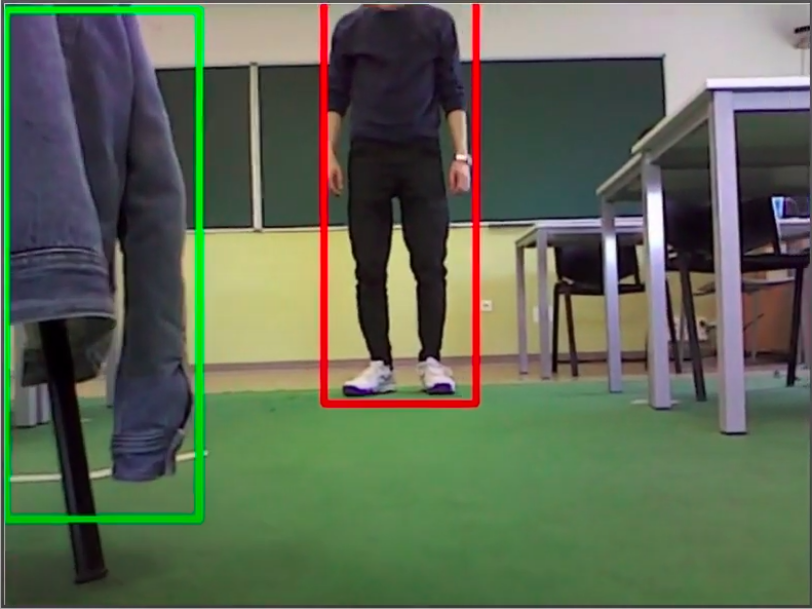
\includegraphics[width=10cm]{imagenes/cap6/tracker.png}
		\end{center}
		\caption[Tracker en el ejercicio Sigue-Persona Real]{Tracker en el ejercicio Sigue-Persona Real}
		\label{fig:tracker_real_follow_person}
	\end{figure}\
	
	\item Implementación del algoritmo VFF. Como la frecuencia de actualización cambia ante la ausencia del simulador, ha sido necesario reajustar los parámetros $\alpha$ y $\beta$ del algoritmo para equilibrar la relación entre la fuerza de atracción y de repulsión. Es recomendable que el párametro $\alpha$ que multiplica a la fuerza de atracción sea mayor que $\beta$ para no perder al objetivo. Sin embargo, tenemos que tener en cuenta que $\beta$ debe estar correctamente ajustado para esquivar con seguridad y suavidad los obstáculos que se encuentre por su camino. Un buen ajuste de parametros permitirá por ejemplo seguir a una persona a través de un pasillo manteniendo la misma distancia con ambas paredes sin importar la colocación de su objetivo. En nuestro caso, los valores de $\alpha$ y $\beta$, comprobados empíricamente, fueron 1.5 y 0.5 respectivamente.
	
	\item Máquina de Estados Finitos. Seguimos usando dos estados maestros: Buscar-Persona y Seguir-Persona. La transición del estado Seguir-Persona a Buscar-Persona estaba determinado por el contador de fallo que iniciamos en el proceso de seguimiento del Tracking. El límite del contador dependerá de los fotogramas por segundo. En el ejercicio Sigue-Persona Simulado, la velocidad de fotogramas era baja por lo tanto el límite era menor, pero en este caso, al haber aumentado la velocidad de refresco, tiene sentido aumentar el límite del contador para que, si perdemos a la persona en un fotograma, podamos seguir guardando el centroide de la última caja de detección candidata.
\end{itemize}\




\subsection{Validación experimental}
\label{subsec:validacion_experimental_real}

Para su validación se realizaron las mismas pruebas que en el ejercicio Sigue-Persona Simulado:\\

\begin{itemize}
	\item Para probar el algoritmo de navegación VFF, pusimos una silla en mitad del escenario (Figura \ref{fig:real_solucion_vff_test} izquierda). Cuando el robot detectaba a su objetivo, empezaba a acercarse, rodeando el obstáculo que tenía a su izquierda. Cada vez que el centroide de la caja de detección se alejaba más del centro de la imagen, mayor era la fuerza de atracción aplicada a la velocidad angular del robot. También, aprovechando el escenario de la \textit{Robocup} en el Laboratorio de Robótica, probamos la navegación a través de un pasillo pudiendo observar que, debido al ajuste correcto de los parámetros de repulsión y atracción, el robot era capaz de seguir a la persona manteniendo la misma distancia con las paredes (Figura \ref{fig:real_solucion_vff_test} - derecha). Una vez que el robot tenía hueco para salir del pasillo, conseguía mantenerse en frente de su objetivo.
	
	\begin{figure} [H]
		\begin{center}
		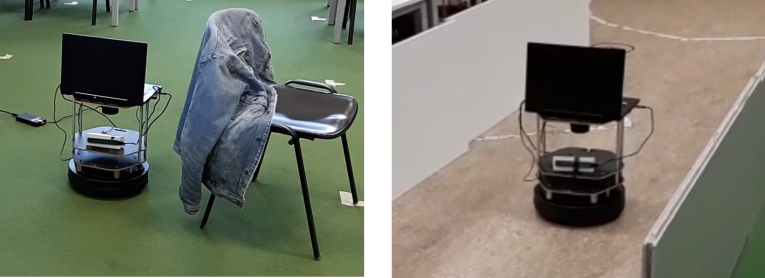
\includegraphics[width=10cm]{imagenes/cap6/real-solucion-vff-test.png}
		\end{center}
		\caption[Solución Sigue-Persona Real: prueba de navegación VFF]{Solución Sigue-Persona Real: prueba de navegación VFF}
		\label{fig:real_solucion_vff_test}
	\end{figure}
	
	\item Durante una de las ejecuciones, después de que el robot detectara a la persona, y la empezara a seguir por el laboratorio, vimos que la detección mostraba un falso positivo en el robot Pepper debido a su aspecto físico parecido al ser humano, además de la chaqueta colocada sobre la silla (Figura \ref{fig:real_solucion_tracking_test}). Como aplicamos el criterio de selección del centroide más cercano al anterior mediante la distancia Euclidea, el robot logra realizar su tarea de seguimiento correctamente.
	
	\begin{figure} [H]
		\begin{center}
		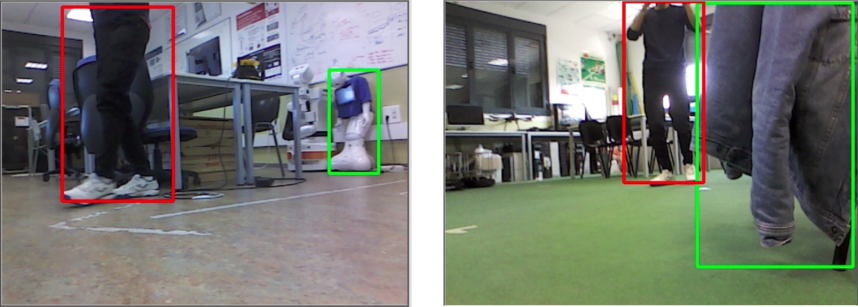
\includegraphics[width=10cm]{imagenes/cap6/real-solucion-tracking-test.png}
		\end{center}
		\caption[Solución Sigue-Persona Real: prueba de seguimiento]{Solución Sigue-Persona Real: prueba de seguimiento}
		\label{fig:real_solucion_tracking_test}
	\end{figure}
\end{itemize}\

El vídeo probando el algoritmo de navegación VFF a través de un pasillo se puede ver a través de este enlace: \url{https://www.youtube.com/watch?v=qIcsjsmKjH8}\\

El vídeo de la ejecución donde mostramos las pruebas descritas esta accesible desde el enlace: \url{https://youtu.be/54Jb4KJwyDM}\\



% -- SECCION VARIANTES
% ----------------------
\section{Variantes alternativas}
\label{sec:variantes_solucion}

La solución mostrada en las secciones \ref{sec:solucion_sigue_personas_simulado} y \ref{sec:solucion_sigue_personas_real} no es la única para abordar la aplicación. Podemos enfocar el problema Sigue-Persona de varias maneras. A continuación indicamos algunas posibles opciones que tuvimos en cuenta antes de llegar a la solución final de referencia:\\

\begin{itemize}
	\item \textbf{Control de velocidad basado en franjas}. En este modelo de seguimiento, dividimos la imagen en franjas y dependiendo de la posición $C_{x}$ del centroide usamos una velocidad angular determinada. En el código \ref{cod:vel_bar} podemos ver un ejemplo de implementación.
\begin{code}[H]
\begin{lstlisting}
vels = [0.3, 0.2, 0.1, 0, -0.1, -0.2, -0.3]	 # vel > 0 === left turn

width = img.shape[1]
step = width/len(vels)

while True:
	# ...
	cx, cy = centroid
	# ...
	
	HAL.setW(vels[int(cx/step)]) # Angular velocity
\end{lstlisting}
\caption{Ejemplo de control de velocidad basado en franjas}
\label{cod:vel_bar}
\end{code}
	Esta fue la primera solución alternativa utilizada, cuyo video se puede ver a través de este enlace: \url{https://www.youtube.com/watch?v=58ckb5fFvrs}\\
	La ventaja de este algoritmo es que el movimiento angular está controlado en un rango elegido por el programador y los cambios de velocidad se realizan de manera suave. La desventaja es que puede provocar pequeñas oscilaciones cuando la caja de detección de la persona se encuentre en el centro de la imagen. Además, hay que tener en cuenta la repulsión del láser, cuya suma puede afectar al movimiento del robot al no existir un vector de atracción.
	
	\item \textbf{Velocidad basada en un controlador PID}. Con un controlador PID bien configurado obtendríamos una respuesta rápida y precisa para no perder a la persona. Su algoritmo de seguimiento sería semejante al ejercicio \textit{Follow Line}\footnote{\textbf{Follow Line}: \url{http://jderobot.github.io/RoboticsAcademy/exercises/AutonomousCars/follow_line/}}. Una desventaja de usar un controlador PID es el hecho de verse afectado a causa de una baja velocidad de fotogramas por segundo provocando oscilaciones constantes. Esta alternativa no tendría en cuenta los obstáculos.
	
	\item \textbf{Detección de color}. Como solución de escape en caso de tener problemas de alto de rendimiento, pensamos la opción de seguir a la persona dependiendo del color de la camiseta. En el caso del hospital pusimos la camiseta del modelo teleoperado de color verde para facilitar la detección. En un escenario real, la persona podría ponerse alguna camiseta de algún color llamativo para facilitar la detección. Para abordar esa solución, tendríamos que seguir estos pasos:
	\begin{enumerate}
		\item Cambiar el espacio de color de la imagen de RGB a HSV\footnote{\textbf{HSV}: \url{https://es.wikipedia.org/wiki/Modelo_de_color_HSV}}. El espacio HSV (Hue, Saturation, Value) facilita la detección de colores.
		\item Obtener el rango HSV de valores mínimo y máximo del color de la camiseta y crear una máscara que la filtre correctamente.
		\item Siendo $p_{i}$ el valor del pixel (0 o 1) de la máscara y $x_i$ las coordenadas del pixel correspondiente, el centroide lo obtendremos de la siguiente manera (ecuacion obtenida de \cite{centroide_ecuacion}):
		\begin{equation*}
		c = \frac{\sum_{i=1}^n\left(p_i \cdot x_i\right)}{\sum_{i=1}^n\left(p_i\right)}
		\end{equation*}
		\item Una vez obtenido el centroide, aplicar el algoritmo VFF igual que en la solución de referencia.
	\end{enumerate}\
	
	En la Figura \ref{fig:color_deteccion} se puede ver un filtro de color verde que utilizamos al principio para el ejercicio Sigue-Persona Simulado:\\
	
\begin{figure} [H]
	\begin{center}
	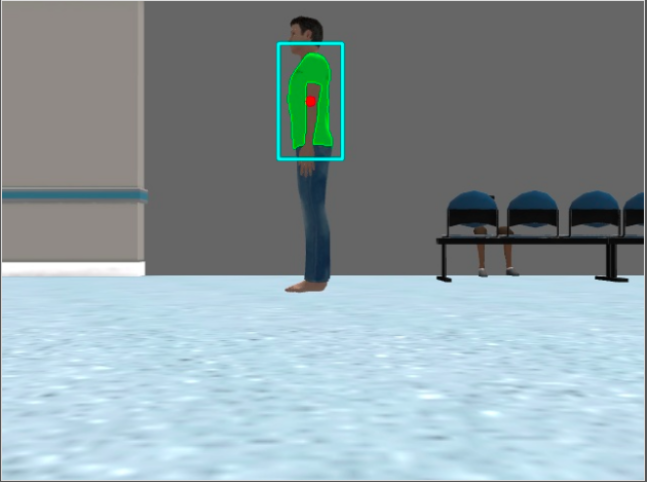
\includegraphics[width=10cm]{imagenes/cap6/deteccion-color.png}
	\end{center}
	\caption[Variante alternativa usando un filtro de color]{Variante alternativa usando un filtro de color}
	\label{fig:color_deteccion}
\end{figure}
	
	La desventaja de esta solución es que la percepción visual basada en filtros de color es frágil porque requiere que la persona a seguir se vista de una determinada manera. Es preferible una percepción basada en RNA porque es mucho más robusta, funciona en un amplio abanico de situaciones y no requiere que la persona se vista de ninguna manera especial.
\end{itemize}



\chapter{Conclusiones}
\label{cap:Conclusiones}

Finalizamos este Trabajo Fin de Grado con las conclusiones y un resumen con los objetivos que hemos alcanzado, además de algunas posibles líneas para futuras derivaciones, investigaciones o ampliaciones que superen las metas alcanzadas en este proyecto

\section{¿Qué ha aportado este trabajo?}
\label{sec:aportaciones}

Una vez terminado el proyecto, hemos logrado alcanzar los objetivos que nos propusimos al principio en el capítulo \ref{cap:capitulo2}:

\begin{enumerate}
	\item Logramos migrar un modelo TurtleBot2 simulado y adaptarlo de ROS Noetic a ROS2 Foxy. Los ficheros fuente se integraron en el repositorio oficial de Custom Robots \footnote{\url{https://github.com/JdeRobot/CustomRobots/tree/foxy-devel}} (rama foxy).
	\item Uno de los objetivos principales conseguidos era entender la infraestructura de Robotics Academy para desarrollar los dos nuevos ejercicios. Actualmente han sido incorporados al conjunto de ejercicios de Robotics Academy: Sigue-Persona Simulado\footnote{\url{http://jderobot.github.io/RoboticsAcademy/exercises/MobileRobots/follow_person}} y Sigue-Persona Real\footnote{\url{http://jderobot.github.io/RoboticsAcademy/exercises/MobileRobots/real_follow_person}}.
	\item Había que diseñar un escenario para el ejercicio Sigue-Persona Simulado, de modo que desarrollamos un \textit{plugin} en ROS2 para controlar una persona simulada en Gazebo usando los botones del teclado a través de la página web. Además incorporamos un hospital, que proporcionaba AWS, en el simulador.
	\item Se ha conseguido integrar por primera vez un \textit{robot real} para un ejercicio de Robotics Academy.
	\item Como último objetivo que marcamos, pudimos proporcionar una \textit{solución} robusta y funcional del algoritmo Sigue-Persona para los dos nuevos ejercicios.
\end{enumerate}

Como aporte adicional, hemos logrado incorporar un modelo de red neuronal óptimo para arquitecturas y software de bajo rendimiento computacional (ejemplo: Docker, Raspberry Pi) para Robotics Academy.

\section{Competencias adquiridas}
\label{sec:competencias}

Durante la realización del TFG se han ido adquiriendo varios conocimientos y competencias sobre distintas tecnologías:

\begin{itemize}
	\item Conocimiento avanzado de Docker: creación de imágenes y uso de contenedores.
	\item Profundización en HTML, CSS y JavaScript.
	\item Ampliación de conocimientos en ROS, ROS2 y ROS Bridge.
	\item Creación de \textit{plugins} para Gazebo.
	\item Ampliación de conocimientos en URDF y Xacro.
	\item Funcionamiento del frontend y backend de Robotics Academy.
	\item Creación de una solución más robusta en el problema robótico de seguir a una persona utilizando algoritmos como \textit{tracking} perceptivo y navegación con \textit{VFF}.
	\item Correcta metodología para trabajar en proyectos de software libre en Github.
\end{itemize}\

\section{Líneas futuras}
\label{sec:lineas_futuras}

Una vez lograda la meta principal de este proyecto, han quedado abiertas varias ramas interesantes para mejorar o investigar:

\begin{itemize}
	\item Sería posible incorporar varios modelos de redes neuronales ligeros parecidos a SSD Inception V2 para ejercicios de \textit{Deep Learning}.
	\item Crear nuevos ejercicios para Robotics Academy usando el TurtleBot2 real o su modelo simulado. Por ejemplo una navegación global en el entorno del Laboratorio de Robótica de la ETSIT-URJC.
	\item Encontrar soporte para cámaras RGB-D en ROS2 Foxy que puedan ser utilizadas en \textit{Robotics Academy} para aprovechar la característica de estimar la distancia de los objetos presentes en los fotogramas o manejar nubes de puntos 3D.
	\item Sería interesante mejorar la solución Sigue-Persona aprovechando la profundidad de una cámara RGB-D. De esta manera, al identificar al objetivo, podríamos lanzar una transformada desde el marco de coordenadas \textit{base\_footprint} y seguir constantemente a la persona gracias a su marco de coordenadas dinámico. Con ello, mejoraríamos en precisión y sería más difícil perder a la persona. También se podría usar la profundidad para determinar el módulo del vector de atracción al utilizar VFF.
\end{itemize}



\printindex \nocite{*}

\printbibliography

\afterpage{\blankpage}


\end{document}